\documentclass[11pt]{article}

% ---- Standard, widely-available packages only (no custom .cls files needed on Overleaf) ----
\usepackage[margin=1in]{geometry}
\usepackage{amsmath,amssymb}
\usepackage{graphicx}
\usepackage{booktabs}
\usepackage[colorlinks=true,citecolor=blue,linkcolor=blue,urlcolor=blue]{hyperref}
\usepackage[numbers,sort&compress]{natbib}
\usepackage{xcolor}
\usepackage{caption}
\usepackage{subcaption}
\usepackage{tikz}
\usetikzlibrary{arrows.meta,fit,positioning}
\usepackage{float}
\usepackage{enumitem}

% No \TODO macro is defined: any open item is left as a LaTeX comment, so nothing
% renders as red placeholder text in the compiled PDF.

\title{Learning Implied Volatility, Not Prices: A Neural-Operator Encoder\\
with a Differentiable Black--Scholes Decoder for SPX Option Pricing}

\author{
Zefang Li \\
\small \texttt{zeke.zefang.li@gmail.com}
}
\date{}

\begin{document}

\maketitle

\begin{abstract}
The Black--Scholes formula is exact once the implied volatility is known. Neural networks estimate
prices, implied volatilities, and hedges. However, how much per-contract conditioning helps remains
unquantified. Here, we learn a \emph{per-contract implied volatility} $\hat\sigma$ and feed it through the closed-form
Black--Scholes (BS) formula, so a plain data loss on $\log(V/K)$ back-propagates through the
analytical pricer, with no learned surrogate. A 2-D Fourier Neural Operator encodes the market state
from one of three inputs (implied-volatility surface, SPX price history, or VIX history), and a
per-query head emits $\hat\sigma$ from each contract's log-moneyness and maturity. On
quote-quality-filtered SPX options (OptionMetrics via WRDS) split 80/10/10 by trade date, three
results follow. Per-query conditioning matters most: one scalar $\hat\sigma$ per market
state rather than per contract collapses put $R^2(\log)$ from 0.978 to about $-0.32$ and
$R^2(\text{price})$ to $-3.090$. The surface-conditioned configuration prices best, $R^2(\log) \approx
0.98$--$0.99$ against $\approx 0.90$--$0.94$ for the historical ones. Autograd partial greeks through
the decoder match closed-form BS at the predicted $\hat\sigma$ to a maximum absolute discrepancy of
$2\times10^{-14}$ (delta) and $2\times10^{-15}$ (vega). Two qualifications apply: the surface
experiment is same-day cross-sectional reconstruction, not forecasting, and the comparison is of whole
input--encoder configurations, not isolated inputs.
\end{abstract}

\section{Introduction}
\label{sec:intro}

Pricing an option is, in principle, a map from market state and contract terms to a price. The
common neural approach regresses that price (or an implied volatility) directly with a general
function approximator, a line of work that begins with~\citet{Hutchinson1994Nonparametric} and is
surveyed by~\citet{RufWang2020Review}. Regressing the price directly throws away structure that is
already known in closed form: under the standard Black--Scholes assumptions, the price is an explicit,
differentiable function of one hard-to-observe quantity, the implied volatility $\sigma$, conditional
on moneyness, maturity, and the dataset-supplied rate and dividend-yield inputs. However, that
literature leaves two empirical questions open about such an architecture: how much a per-contract
$\hat\sigma$ buys relative to a market-state-only scalar $\hat\sigma$, and which of three market-state
inputs (an implied-volatility surface, an SPX price history, or a VIX history) prices best when the
architecture, dataset, and date split are held fixed. Neither has been quantified side by side on SPX
options~\citep{RufWang2020Review}. Here, we train
a network to predict only $\sigma$---more precisely, a per-contract estimate $\hat\sigma$ conditioned
on the broader market state---and recover the price analytically through the BS formula. Because BS is
composed of differentiable primitives ($\exp$, $\mathrm{erf}$, $\sqrt{\cdot}$), the training loss on
$\log(V/K)$ back-propagates through the closed-form decoder into the network exactly as it would
through any other differentiable layer; no learned pricing surrogate is needed.

Two structural properties follow from this design, and we state them at the precision the checks in
this paper actually support. First, conditional on a fixed predicted $\hat\sigma$, the decoder returns
the closed-form BS price, respects its single-contract static no-arbitrage bounds, and has the
corresponding analytical partial derivatives. This is a \emph{pointwise, frozen-$\hat\sigma$}
Black--Scholes-consistency property, not a claim about the total learned map: $\hat\sigma$ itself
varies with the query $(\log(S/K), T)$, so the composed map from market state and contract terms to
price need not satisfy the BS PDE, whose derivation assumes a volatility that does not depend on
strike or maturity~\citep{Dupire1994Smile}. Nor is it a claim that the full predicted surface is
arbitrage-free---because $\hat\sigma$ is fit independently for each query, nothing in the architecture
guarantees calendar-spread or butterfly consistency \emph{across} the predicted $(K,T)$ surface, and
we do not check this here. Second, every greek we report is the closed-form BS partial derivative
evaluated at the predicted $\hat\sigma$, holding $\hat\sigma$ fixed---an \emph{analytic partial
greek}, not the total sensitivity of the learned system, which would include an additional
$\partial\hat\sigma/\partial S \cdot \text{vega}$ term that a frozen-$\hat\sigma$ check cannot see.

\paragraph{Contributions.} This is an empirical, application-focused study rather than a new-method
paper: the differentiable-BS-decoder idea is not novel to the machine learning or quantitative finance
communities (Section~\ref{sec:related}). We make three specific, evaluated claims.

\begin{enumerate}[leftmargin=*]
\item \textbf{Per-query volatility conditioning is what makes the smile/skew learnable.} We compare
the full per-query architecture against a scalar-$\hat\sigma$ ablation that predicts one volatility per
market state (flat-vol BS, no smile or skew) with everything else held fixed. The gap is large and, for
puts, qualitative: removing per-query conditioning drives put $R^2(\text{price})$ negative
(Section~\ref{sec:results-ablation}).
\item \textbf{We quantify which of three candidate market-state input--encoder configurations prices
best.} Comparing an implied-volatility-surface encoder against SPX-price-history and VIX-history
encoders, the surface configuration wins by a wide and consistent margin on both option types and both
head architectures (Section~\ref{sec:results-branch}). Two qualifications travel with this result.
(a) The surface branch is fed OptionMetrics' own same-day standardized volatility surface, derived
from that trading day's option quotes; the date-based split rules out cross-date leakage but not this
same-day dependence, so that branch demonstrates same-day cross-sectional reconstruction conditional
on an observed surface rather than independent price discovery. The SPX-history and VIX-history
tensors are 21-trading-day windows ending on the target trade date and therefore include that day's
underlying and VIX closes; their same-day dependence on the option market is weaker and far
lower-dimensional than the surface branch's (SPX history has none directly, only the same-day
underlying close; VIX is a single scalar index that Cboe computes from contemporaneous SPX option
quotations), but it is not zero. (b) The three encoders are \emph{not} parameter-matched---the
flattened FNO output is projected to the latent vector by two dense layers, and the first of them,
whose input width scales with the grid, dominates the count: it holds 766{,}080 parameters (weights
and bias) for the $11{\times}17$ surface grid, 430{,}208 for
the $21{\times}5$ SPX-history grid, and 344{,}192 for the $21{\times}4$ VIX-history grid, so input
content, timing, normalization, grid size, and capacity all vary together and the comparison is
between whole configurations, not raw inputs (Section~\ref{sec:limitations}).
\item \textbf{The BS decoder gives verified derivative consistency at the predicted $\hat\sigma$.} We
compare autograd-computed delta and vega through the decoder against the closed-form BS expressions at
the same $\hat\sigma$ and find agreement at float64 machine precision, confirming the decoder is
implemented and differentiated correctly (Section~\ref{sec:results-greeks}).
\end{enumerate}

We additionally report a comparison between the two per-query head designs used throughout (an MLP
head and a DeepONet branch--trunk readout). The observed differences are small relative to the
seed-to-seed variation we measure, and three seeds are insufficient to rank the two architectures, so
we do not treat this as a fourth contribution or a ranking claim (Section~\ref{sec:results-ab}).

\section{Related work}
\label{sec:related}

\paragraph{Option pricing theory.} The closed-form Black--Scholes formula~\citep{BlackScholes1973}
and its rational-pricing derivation~\citep{Merton1973} are the analytical decoder we build on; we make
no claim to extend or revise the theory itself, only to use it as a differentiable output layer.

\paragraph{Neural networks for option pricing.} \citet{Hutchinson1994Nonparametric} introduced
nonparametric learning networks for pricing and hedging derivative securities, and~\citet{RufWang2020Review}
survey the three decades of work that followed. \citet{Culkin2017} trained a feed-forward network to
reproduce Black--Scholes prices directly, establishing that a network can learn the BS pricing function
to high accuracy as a numerical approximation. \citet{Horvath2021DeepVol} instead used networks to
accelerate calibration of (rough) stochastic volatility models against market implied volatility
surfaces. Our design differs from all of these in keeping the BS formula itself analytical and training the
network only to output its one free parameter, $\hat\sigma$, per contract; we do not train a network to
approximate BS itself, and we do not calibrate a parametric stochastic volatility model.

\paragraph{Implied-volatility-surface-conditioned neural pricing.} Closest in spirit to our surface
branch,~\citet{Wiedemann2025OpDeepSmoothing} use a neural operator to map raw, irregularly observed
option quotes directly to a smoothed implied-volatility surface, and~\citet{Ding2025DLIVSurfaces}
compress observed market volatility surfaces with a variational autoencoder and price contracts from
the resulting latent code together with strike and maturity. \citet{Ackerer2020DeepSmoothing} fit the
implied-volatility surface itself with a neural network trained on the observed quotes, adding soft
no-arbitrage penalties on the predicted surface to the loss. All three condition on contemporaneous
option-market information, as our surface-branch experiment does. Our contribution relative to them is not the
conditioning itself but the analytical BS output layer (the network emits only $\hat\sigma$) and the
side-by-side comparison of that surface input against purely historical inputs on the same
architecture, dataset, and split.

\paragraph{Physics-informed and structure-constrained approaches.} Physics-informed neural
networks~\citep{Raissi2019PINN} enforce a governing PDE via a soft penalty term added to the training loss,
originally in a physics setting and subsequently adapted to option pricing and calibration problems by
other authors. Our architecture reaches a related but weaker property---at a frozen predicted
$\hat\sigma$, the closed-form BS price and its single-contract static no-arbitrage bounds at each
queried contract---structurally, by construction of the decoder, rather than via an auxiliary loss
term; Section~\ref{sec:method-decoder} states precisely what this guarantees and does not guarantee.

\paragraph{Neural operators.} The market-state encoder is a 2-D Fourier Neural
Operator~\citep{Li2021FNO}. We also use a DeepONet-style branch--trunk readout~\citep{Lu2021DeepONet} as an
alternative per-query head, dotting a market-state branch vector against a trunk network evaluated at
each contract's $(\log$-moneyness$, T)$ query. \citet{NoguerIAlonso2026DerivInformed} train
operator-learning surrogates for finance against both prices and directional derivatives, and draw the
same distinction we rely on in Sections~\ref{sec:method-decoder} and~\ref{sec:results-greeks}: a
surrogate that matches prices need not match their sensitivities, so derivative consistency is a
separate property that must be established on its own terms rather than inferred from pricing
accuracy.

\paragraph{Classical implied-volatility surface modeling.} SVI~\citep{Gatheral2004SVI} and its
arbitrage-free extension SSVI~\citep{GatherJacquier2014SSVI} are standard practitioner
parameterizations of the implied-volatility smile; we use spline and nearest-neighbor interpolation of
the observed surface as one of our practitioner baselines (Section~\ref{sec:baselines-method}) rather
than fitting SVI directly.

\paragraph{Quote-quality filtering.} Excluding option observations that violate static no-arbitrage
bounds prior to model fitting has precedent in the literature:~\citet{Buechner2021Factor} filter
option return panels on data-quality grounds in an asset-pricing context, and~\citet{Cohen2020Arbitrage}
both detect and repair arbitrage violations in traded option price data, cautioning that outright
removal (as opposed to repair) discards information. Our dataset filter (Section~\ref{sec:data-filter})
follows the removal approach, with the caveat these authors raise explicitly noted.

\section{Method}
\label{sec:method}

\subsection{The inverse implied-volatility problem}
\label{sec:method-inverse}
Given an observed normalized option price $V/K$ for a contract with log-moneyness $m = \log(S/K)$,
maturity $T$, risk-free rate $r$, and dividend yield $q$, the implied volatility $\sigma$ is the value
that makes the BS formula reproduce the observed price. We train an estimator $\hat\sigma$ of this
quantity, conditioned on the broader market state, and price through BS. The training target is
$\log(V/K)$ rather than $V/K$ itself, since option prices span several orders of magnitude across
moneyness and maturity.

\subsection{Market-state encoder}
\label{sec:method-encoder}
The market state is encoded by a 2-D Fourier Neural Operator~\citep{Li2021FNO}: four spectral
convolution blocks with $1{\times}1$-convolution skip connections and SiLU activations, flattened and
projected to a 128-dimensional latent vector. We evaluate three candidate market-state inputs, one per
encoder instance, each reshaped from its native 1-D form to a 2-D grid inside the encoder.

The \textbf{implied-volatility surface} input is OptionMetrics' standardized volatility
surface~\citep{OptionMetrics2026Surface} for the \emph{same} trade date, on an $11 \times 17$ (maturity
$\times$ delta) grid. This input is derived from that day's own option quotes
(Section~\ref{sec:data-surface}), so this branch is conditioned on contemporaneous cross-sectional
information rather than on strictly prior information. The \textbf{SPX price history} input is 21
trading days of SPX OHLCV data, a $21 \times 5$ grid, each row divided by the window's final close (and
volume by the final volume); the window \emph{ends on} the target trade date rather than the day
before it, so the final row is that day's own OHLCV and that day's close is the normalization
denominator for the whole tensor. The \textbf{VIX history} input is 21 trading days of CBOE VIX OHLC
data, a $21 \times 4$ grid, likewise ending on the target trade date and normalized the same way: each
value is divided by the window's final (i.e.\ same-day) VIX close. This representation is therefore
scale-free and retains only the \emph{shape} of the recent VIX path; the absolute VIX level is not
visible to that encoder.

Neither historical input is a strictly-prior-information input: both windows include the target trade
date, and VIX is itself computed by Cboe from a strip of contemporaneous SPX option
quotations~\citep{Cboe2026VIXFAQ}, so even the VIX branch is not free of same-day option-market information. What
separates these branches from the surface branch is the amount and directness of that information---a
single scalar index (further reduced to a shape by the normalization) versus the full standardized
$11 \times 17$ implied volatility surface---not its presence or absence.

The flattened FNO output is projected to the latent vector by two dense layers, a flatten-to-128 layer
whose input width is proportional to the grid size followed by a fixed 128-to-latent layer, so the
three encoders differ in parameter count. The first layer dominates that difference and is the one the
published counts refer to: including its bias it holds 766{,}080 parameters for the surface grid,
430{,}208 for SPX history, and 344{,}192 for VIX history, while the second layer is identical across
all three branches. The branch comparison in Section~\ref{sec:results-branch} is consequently not a
capacity-controlled comparison, and we read it accordingly (Section~\ref{sec:limitations}).

\subsection{Per-query volatility head}
\label{sec:method-head}
The market-state latent vector feeds a per-query head that additionally takes each contract's
$(\log$-moneyness$, T)$ query and outputs $\hat\sigma$ for that specific contract, not one scalar per
market state. We compare two interchangeable head designs, both with hidden width 128 acting on the
same 128-dimensional latent vector. Architecture A (MLP head) is an MLP on the concatenation of the
latent vector and the query $(\log$-moneyness$, T)$, followed by a softplus to keep $\hat\sigma$
positive. Architecture B (DeepONet) is a DeepONet-style branch--trunk readout~\citep{Lu2021DeepONet}:
the FNO output is the branch vector, a trunk MLP embeds $(\log$-moneyness$, T)$, and $\hat\sigma$ is a
softplus of their dot product plus a bias, with a small positive floor added for numerical stability.

Per-query conditioning is the central design choice of this paper: because $\hat\sigma$ depends on the
specific contract being priced, not only on the market state, the model can in principle recover the
volatility smile/skew, which a market-state-only $\hat\sigma$ cannot. Section~\ref{sec:results-ablation}
isolates the effect of this choice.

\subsection{Differentiable Black--Scholes decoder}
\label{sec:method-decoder}
A closed-form BS pricing function maps $(\log$-moneyness$, T, r, q, \hat\sigma)$ to the normalized
price $V/K$ using only differentiable primitives ($\exp$, $\mathrm{erf}$, $\sqrt{\cdot}$). Gradients of
the data loss on $\log(V/K)$ flow through this decoder into the encoder and head exactly as through any
other differentiable layer; there is no learned or neural pricing surrogate anywhere in the forward
pass. Figure~\ref{fig:f1} summarizes the full forward pass.

Two properties follow directly from using an analytical decoder. First, every reported greek is the
closed-form BS partial derivative evaluated at the predicted $\hat\sigma$, holding $\hat\sigma$ fixed.
We verify this numerically in Section~\ref{sec:results-greeks} by comparing autograd through the
decoder against the closed-form expressions; this checks decoder correctness, not the total
(sticky-strike) sensitivity of the learned system, which would additionally involve $\partial \hat\sigma
/ \partial S$. Second, conditional on a fixed predicted $\hat\sigma$, the decoder returns the
closed-form BS price, respects its single-contract static no-arbitrage bounds, and has the
corresponding analytical partial derivatives---a property of the frozen-$\hat\sigma$ mapping only.
It is not a claim that the total learned map solves the BS PDE: the predicted $\hat\sigma$ is a
function of the query $(\log(S/K), T)$, whereas the BS PDE is derived under a volatility that does not
vary with strike or maturity, so the composed map need not satisfy it. Nor does the pointwise property
guarantee calendar-spread or butterfly consistency across the full predicted $(K,T)$ surface, since
$\hat\sigma$ is estimated independently per query; we do not run a surface-wide arbitrage
violation-rate check in this paper.

A third property is a limit rather than a guarantee. As $T \to 0$ the Black--Scholes price converges to
the discounted forward intrinsic value for every $\sigma$, so at exact expiry the theoretical price
carries no information about volatility and the implied volatility is unidentified there. The
settlement-aware maturity filter of Section~\ref{sec:data-maturity}, which retains only contracts with
strictly more than 24 hours remaining to settlement, excludes this case from the sample. The
implementation is not exactly $\hat\sigma$-independent at $T{=}0$: it evaluates
$\sqrt{\mathrm{clamp}(T, 10^{-10})}$, clamping the maturity before taking the square root rather than
clamping the square root itself, and therefore retains a residual $\hat\sigma$ dependence of order
$10^{-5}$ in a vanishing band around the money: a synthetic exact-$T{=}0$ probe of the decoder finds a
maximum price spread over $\hat\sigma$ of $1.2\times10^{-5}$ in $V/K$ units
(\texttt{results/diagnostics\_tail\_v5.json}). No contract in this dataset reaches that regime.

\begin{figure}[t]
\centering
\resizebox{\linewidth}{!}{% F1 -- architecture / forward-pass diagram.
% Standalone TikZ, included via % F1 -- architecture / forward-pass diagram.
% Standalone TikZ, included via % F1 -- architecture / forward-pass diagram.
% Standalone TikZ, included via \input{figures/fig_f1_architecture} inside a
% figure environment in main.tex. Matches report.md Sec.3 (Method) exactly:
%   one of three branch inputs -> FNO encoder -> latent market-state vector
%   -> per-query vol head (latent + (log-moneyness, T)) -> sigma-hat
%   -> analytical Black-Scholes decoder -> price (V/K).
% The decoder signature is bs_normalized_price(log_moneyness, T, r, q, sigma),
% so it takes five inputs: the contract query and (r, q) go into it directly,
% alongside sigma-hat from the head.
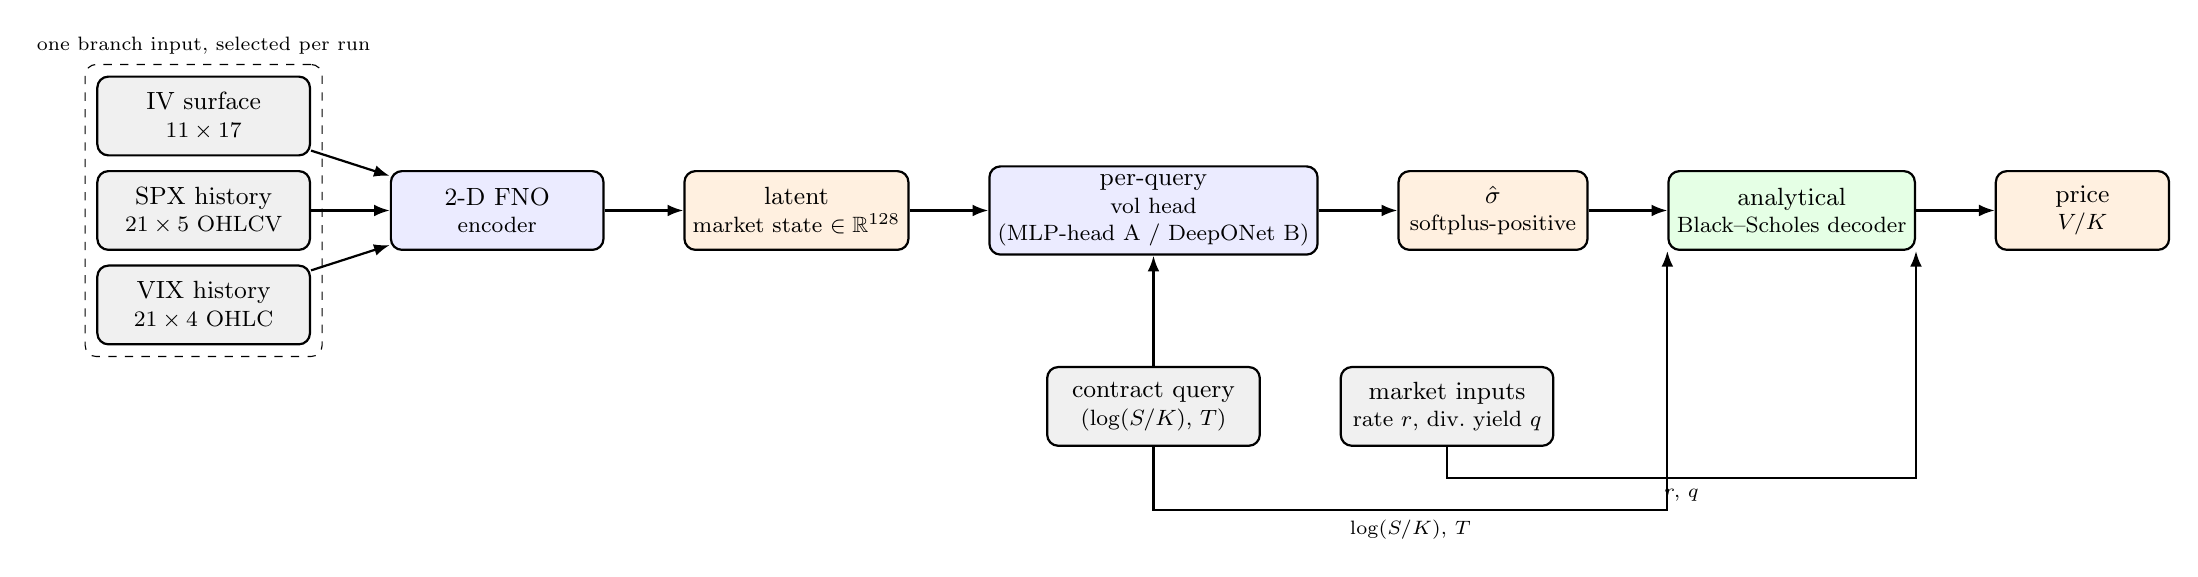
\begin{tikzpicture}[
    font=\small,
    node distance=8mm and 10mm,
    box/.style={draw, thick, rounded corners, align=center, minimum height=10mm, inner sep=3pt},
    inputbox/.style={box, fill=gray!12, minimum width=27mm},
    procbox/.style={box, fill=blue!8, minimum width=27mm},
    vecbox/.style={box, fill=orange!12, minimum width=24mm},
    decbox/.style={box, fill=green!10, minimum width=27mm},
    arrow/.style={-{Latex[length=2mm]}, thick}
]

% --- three interchangeable branch inputs (stacked) ---
\node[inputbox] (in1) at (0, 12mm)  {IV surface\\[-1pt]\footnotesize $11\times17$};
\node[inputbox] (in2) at (0, 0)     {SPX history\\[-1pt]\footnotesize $21\times5$ OHLCV};
\node[inputbox] (in3) at (0,-12mm)  {VIX history\\[-1pt]\footnotesize $21\times4$ OHLC};

\node[draw, dashed, rounded corners, fit=(in1)(in2)(in3), inner sep=4pt, label={[font=\scriptsize]above:one branch input, selected per run}] (inputgroup) {};

% --- FNO encoder ---
\node[procbox, right=of in2] (fno) {2-D FNO\\[-1pt]\footnotesize encoder};

% --- latent vector ---
\node[vecbox, right=of fno] (latent) {latent\\[-1pt]\footnotesize market state $\in\mathbb{R}^{128}$};

% --- per-query head ---
\node[procbox, right=of latent] (head) {per-query\\[-1pt]\footnotesize vol head\\[-1pt]\footnotesize (MLP-head A / DeepONet B)};

% --- contract terms: the query (log-moneyness, T) feeds the head AND, together with
%     the observed rate and dividend yield (r, q), the BS decoder directly.
\node[inputbox, below=14mm of head, minimum width=27mm] (query) {contract query\\[-1pt]\footnotesize $(\log(S/K),\,T)$};
\node[inputbox, right=10mm of query, minimum width=27mm] (rq) {market inputs\\[-1pt]\footnotesize rate $r$, div.\ yield $q$};

% --- sigma hat ---
\node[vecbox, right=of head] (sigma) {$\hat\sigma$\\[-1pt]\footnotesize softplus-positive};

% --- BS decoder ---
\node[decbox, right=of sigma] (bs) {analytical\\[-1pt]\footnotesize Black--Scholes decoder};

% --- price output ---
\node[vecbox, right=of bs, minimum width=22mm] (price) {price\\[-1pt]\footnotesize $V/K$};

% arrows
\draw[arrow] (in1) -- (fno);
\draw[arrow] (in2) -- (fno);
\draw[arrow] (in3) -- (fno);
\draw[arrow] (fno) -- (latent);
\draw[arrow] (latent) -- (head);
\draw[arrow] (query) -- (head);
\draw[arrow] (head) -- (sigma);
\draw[arrow] (sigma) -- (bs);
% the decoder also consumes the contract terms directly, not only sigma-hat
\draw[arrow] (query.south) -- ++(0,-8mm) -| (bs.south west)
    node[pos=0.25, below, font=\scriptsize] {$\log(S/K),\,T$};
\draw[arrow] (rq.south) -- ++(0,-4mm) -| (bs.south east)
    node[pos=0.25, below, font=\scriptsize] {$r,\,q$};
\draw[arrow] (bs) -- (price);

\end{tikzpicture}
 inside a
% figure environment in main.tex. Matches report.md Sec.3 (Method) exactly:
%   one of three branch inputs -> FNO encoder -> latent market-state vector
%   -> per-query vol head (latent + (log-moneyness, T)) -> sigma-hat
%   -> analytical Black-Scholes decoder -> price (V/K).
% The decoder signature is bs_normalized_price(log_moneyness, T, r, q, sigma),
% so it takes five inputs: the contract query and (r, q) go into it directly,
% alongside sigma-hat from the head.
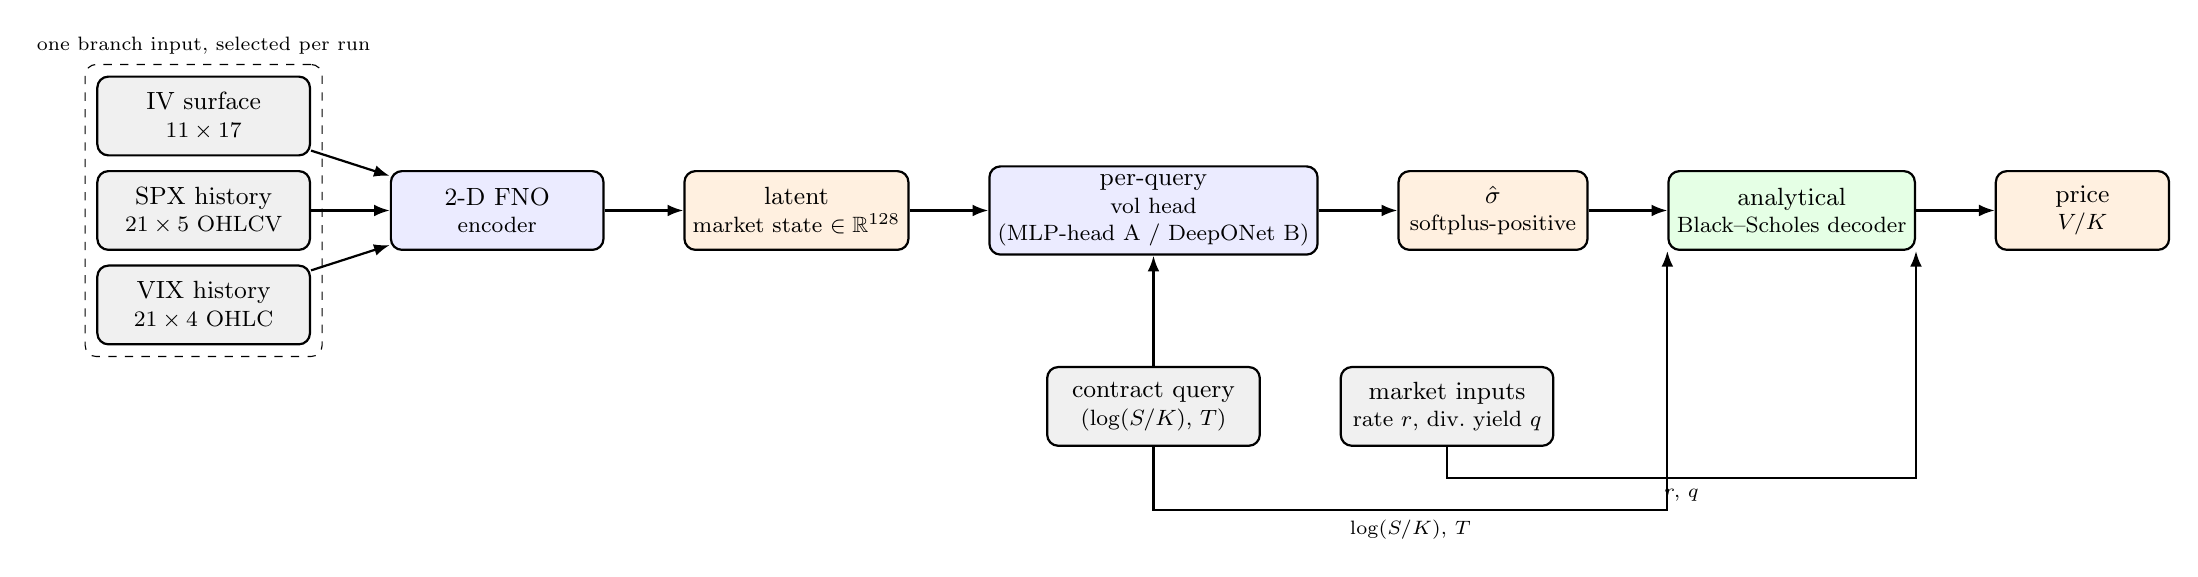
\begin{tikzpicture}[
    font=\small,
    node distance=8mm and 10mm,
    box/.style={draw, thick, rounded corners, align=center, minimum height=10mm, inner sep=3pt},
    inputbox/.style={box, fill=gray!12, minimum width=27mm},
    procbox/.style={box, fill=blue!8, minimum width=27mm},
    vecbox/.style={box, fill=orange!12, minimum width=24mm},
    decbox/.style={box, fill=green!10, minimum width=27mm},
    arrow/.style={-{Latex[length=2mm]}, thick}
]

% --- three interchangeable branch inputs (stacked) ---
\node[inputbox] (in1) at (0, 12mm)  {IV surface\\[-1pt]\footnotesize $11\times17$};
\node[inputbox] (in2) at (0, 0)     {SPX history\\[-1pt]\footnotesize $21\times5$ OHLCV};
\node[inputbox] (in3) at (0,-12mm)  {VIX history\\[-1pt]\footnotesize $21\times4$ OHLC};

\node[draw, dashed, rounded corners, fit=(in1)(in2)(in3), inner sep=4pt, label={[font=\scriptsize]above:one branch input, selected per run}] (inputgroup) {};

% --- FNO encoder ---
\node[procbox, right=of in2] (fno) {2-D FNO\\[-1pt]\footnotesize encoder};

% --- latent vector ---
\node[vecbox, right=of fno] (latent) {latent\\[-1pt]\footnotesize market state $\in\mathbb{R}^{128}$};

% --- per-query head ---
\node[procbox, right=of latent] (head) {per-query\\[-1pt]\footnotesize vol head\\[-1pt]\footnotesize (MLP-head A / DeepONet B)};

% --- contract terms: the query (log-moneyness, T) feeds the head AND, together with
%     the observed rate and dividend yield (r, q), the BS decoder directly.
\node[inputbox, below=14mm of head, minimum width=27mm] (query) {contract query\\[-1pt]\footnotesize $(\log(S/K),\,T)$};
\node[inputbox, right=10mm of query, minimum width=27mm] (rq) {market inputs\\[-1pt]\footnotesize rate $r$, div.\ yield $q$};

% --- sigma hat ---
\node[vecbox, right=of head] (sigma) {$\hat\sigma$\\[-1pt]\footnotesize softplus-positive};

% --- BS decoder ---
\node[decbox, right=of sigma] (bs) {analytical\\[-1pt]\footnotesize Black--Scholes decoder};

% --- price output ---
\node[vecbox, right=of bs, minimum width=22mm] (price) {price\\[-1pt]\footnotesize $V/K$};

% arrows
\draw[arrow] (in1) -- (fno);
\draw[arrow] (in2) -- (fno);
\draw[arrow] (in3) -- (fno);
\draw[arrow] (fno) -- (latent);
\draw[arrow] (latent) -- (head);
\draw[arrow] (query) -- (head);
\draw[arrow] (head) -- (sigma);
\draw[arrow] (sigma) -- (bs);
% the decoder also consumes the contract terms directly, not only sigma-hat
\draw[arrow] (query.south) -- ++(0,-8mm) -| (bs.south west)
    node[pos=0.25, below, font=\scriptsize] {$\log(S/K),\,T$};
\draw[arrow] (rq.south) -- ++(0,-4mm) -| (bs.south east)
    node[pos=0.25, below, font=\scriptsize] {$r,\,q$};
\draw[arrow] (bs) -- (price);

\end{tikzpicture}
 inside a
% figure environment in main.tex. Matches report.md Sec.3 (Method) exactly:
%   one of three branch inputs -> FNO encoder -> latent market-state vector
%   -> per-query vol head (latent + (log-moneyness, T)) -> sigma-hat
%   -> analytical Black-Scholes decoder -> price (V/K).
% The decoder signature is bs_normalized_price(log_moneyness, T, r, q, sigma),
% so it takes five inputs: the contract query and (r, q) go into it directly,
% alongside sigma-hat from the head.
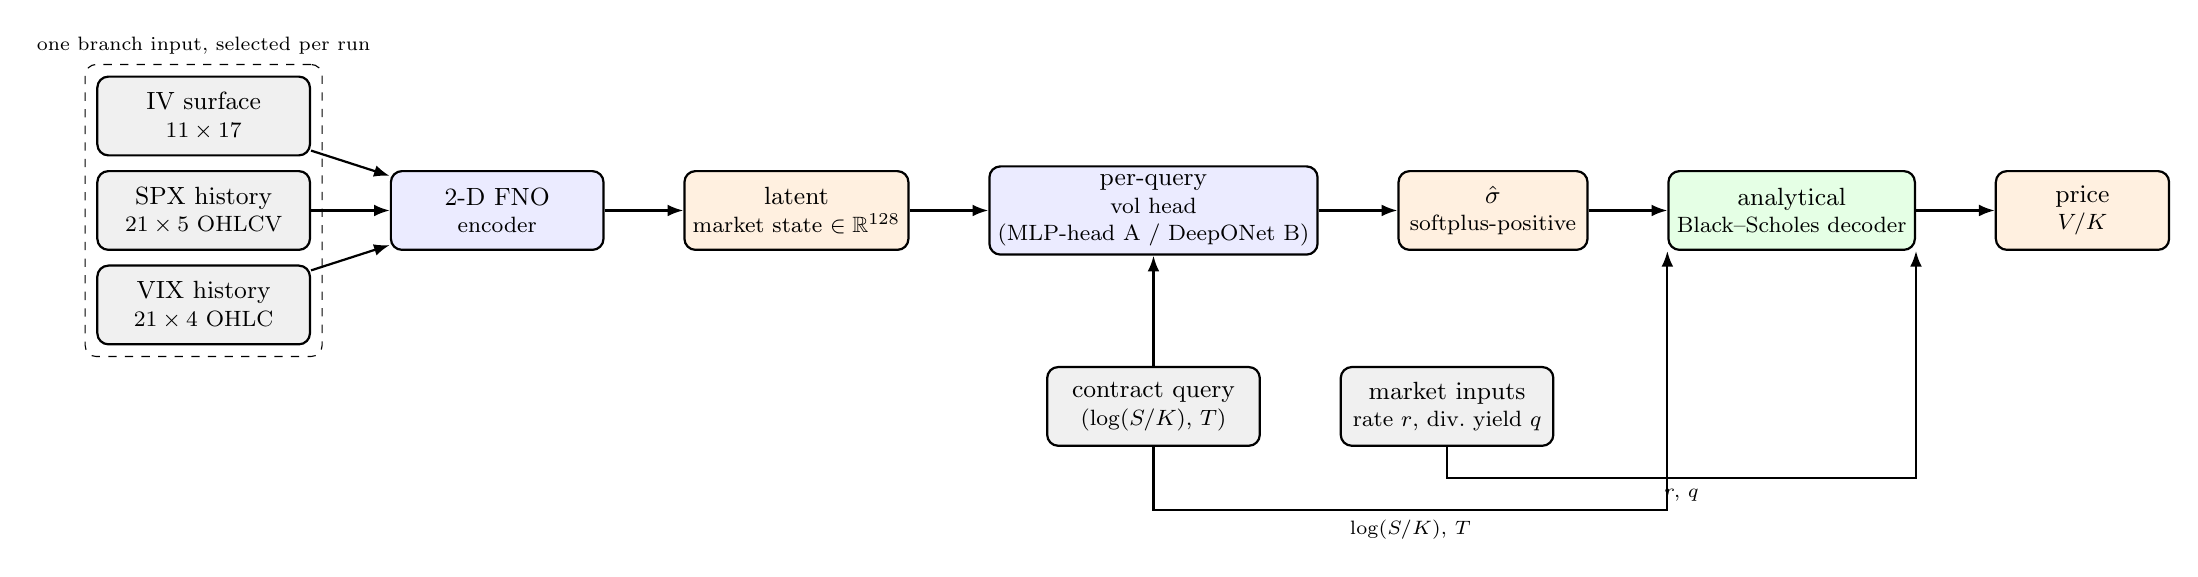
\begin{tikzpicture}[
    font=\small,
    node distance=8mm and 10mm,
    box/.style={draw, thick, rounded corners, align=center, minimum height=10mm, inner sep=3pt},
    inputbox/.style={box, fill=gray!12, minimum width=27mm},
    procbox/.style={box, fill=blue!8, minimum width=27mm},
    vecbox/.style={box, fill=orange!12, minimum width=24mm},
    decbox/.style={box, fill=green!10, minimum width=27mm},
    arrow/.style={-{Latex[length=2mm]}, thick}
]

% --- three interchangeable branch inputs (stacked) ---
\node[inputbox] (in1) at (0, 12mm)  {IV surface\\[-1pt]\footnotesize $11\times17$};
\node[inputbox] (in2) at (0, 0)     {SPX history\\[-1pt]\footnotesize $21\times5$ OHLCV};
\node[inputbox] (in3) at (0,-12mm)  {VIX history\\[-1pt]\footnotesize $21\times4$ OHLC};

\node[draw, dashed, rounded corners, fit=(in1)(in2)(in3), inner sep=4pt, label={[font=\scriptsize]above:one branch input, selected per run}] (inputgroup) {};

% --- FNO encoder ---
\node[procbox, right=of in2] (fno) {2-D FNO\\[-1pt]\footnotesize encoder};

% --- latent vector ---
\node[vecbox, right=of fno] (latent) {latent\\[-1pt]\footnotesize market state $\in\mathbb{R}^{128}$};

% --- per-query head ---
\node[procbox, right=of latent] (head) {per-query\\[-1pt]\footnotesize vol head\\[-1pt]\footnotesize (MLP-head A / DeepONet B)};

% --- contract terms: the query (log-moneyness, T) feeds the head AND, together with
%     the observed rate and dividend yield (r, q), the BS decoder directly.
\node[inputbox, below=14mm of head, minimum width=27mm] (query) {contract query\\[-1pt]\footnotesize $(\log(S/K),\,T)$};
\node[inputbox, right=10mm of query, minimum width=27mm] (rq) {market inputs\\[-1pt]\footnotesize rate $r$, div.\ yield $q$};

% --- sigma hat ---
\node[vecbox, right=of head] (sigma) {$\hat\sigma$\\[-1pt]\footnotesize softplus-positive};

% --- BS decoder ---
\node[decbox, right=of sigma] (bs) {analytical\\[-1pt]\footnotesize Black--Scholes decoder};

% --- price output ---
\node[vecbox, right=of bs, minimum width=22mm] (price) {price\\[-1pt]\footnotesize $V/K$};

% arrows
\draw[arrow] (in1) -- (fno);
\draw[arrow] (in2) -- (fno);
\draw[arrow] (in3) -- (fno);
\draw[arrow] (fno) -- (latent);
\draw[arrow] (latent) -- (head);
\draw[arrow] (query) -- (head);
\draw[arrow] (head) -- (sigma);
\draw[arrow] (sigma) -- (bs);
% the decoder also consumes the contract terms directly, not only sigma-hat
\draw[arrow] (query.south) -- ++(0,-8mm) -| (bs.south west)
    node[pos=0.25, below, font=\scriptsize] {$\log(S/K),\,T$};
\draw[arrow] (rq.south) -- ++(0,-4mm) -| (bs.south east)
    node[pos=0.25, below, font=\scriptsize] {$r,\,q$};
\draw[arrow] (bs) -- (price);

\end{tikzpicture}
}
\caption{\textbf{Forward pass.} One of three candidate market-state inputs (implied-volatility surface,
SPX price history, or VIX history) is encoded by a 2-D FNO into a shared latent vector. A per-query
volatility head (architecture A: MLP head, or architecture B: DeepONet branch--trunk) combines the
latent vector with a contract-specific query $(\log(S/K), T)$ to produce $\hat\sigma$. The analytical
Black--Scholes decoder takes five inputs---$\log(S/K)$, $T$, the rate $r$, the dividend yield $q$,
and $\hat\sigma$---and returns the normalized price $V/K$; the first four are observed contract and
market data routed to the decoder directly, and only $\hat\sigma$ comes from the network. The pricing
function itself is fixed and differentiable.}
\label{fig:f1}
\end{figure}

\subsection{Loss}
\label{sec:method-loss}
Training minimizes plain mean-squared error on $\log(V/K)$, computed as $\log(\mathrm{clamp}(V/K,
10^{-8}))$ for numerical stability. There is no auxiliary PDE, arbitrage, or BS-anchor penalty term. We
do not claim such terms would be redundant: the pointwise consistency of Section~\ref{sec:method-decoder}
says nothing about calendar-spread or butterfly consistency across the predicted surface, which is
exactly what a soft arbitrage penalty of the kind used by~\citet{Ackerer2020DeepSmoothing} would
target. The plain data loss is used because it was sufficient for the questions this paper asks and
keeps the training objective free of tuned penalty weights; adding and evaluating a surface-wide
calendar-spread and butterfly penalty on the predicted $(K,T)$ grid is left to future work.

\section{Data}
\label{sec:data}

We use SPX index options from OptionMetrics, accessed via WRDS, covering 2015-02-02 through
2025-08-29. European exercise removes the early-exercise complication, and BS is used as the analytical
decoder. Contracts are filtered to those with nonzero traded volume.

\subsection{The implied-volatility-surface input and its same-day dependence}
\label{sec:data-surface}
The surface branch input is OptionMetrics' standardized volatility
surface~\citep{OptionMetrics2026Surface}: an $11 \times 17$ grid of interpolated implied volatilities over
eleven fixed maturities (10--730 calendar days) and seventeen fixed BS spot-delta points ($+10$ to
$+90$ for calls, $-90$ to $-10$ for puts). Preprocessing joins this surface to the option targets on
\emph{the same trade date}. Because~\citet{OptionMetrics2026Surface} construct the surface by
interpolating that day's own option implied volatilities, the input can share information with the
population of quotes being priced: the date-based split described below assigns each trade date
entirely to one split, but it does not and cannot remove this within-date dependence. Accordingly, the
surface-branch experiment should be read as out-of-time (date-split), same-day cross-sectional
reconstruction conditional on an observed surface---a nowcasting task---and not as independent
price discovery or as forecasting.

The SPX-history and VIX-history inputs are built from a 21-trading-day OHLC(V) window that \emph{ends
on} the target trade date, so they are not lagged-only inputs: the final row is the trade date's own
bar, and that day's close is the denominator used to normalize the entire tensor. Their same-day
dependence on the \emph{option} market is nevertheless much weaker than the surface branch's. SPX
history sees only the same-day underlying price; VIX history sees a single scalar index, which Cboe
computes from a weighted strip of contemporaneous SPX option bid/ask
quotations~\citep{Cboe2026VIXFAQ}, further reduced by this representation to a path shape. The ordering in
directness of same-day option-market information is therefore surface $>$ VIX history $>$ SPX history,
with only the surface branch receiving the day's full cross-section of implied volatilities.

\subsection{Maturity and contract-identity handling}
\label{sec:data-maturity}
Each contract's maturity is computed on a settlement-aware basis: AM-settled contracts lose the 6.5
hours between the prior end-of-day quote and the 9:30 ET opening settlement print, and we retain only
contracts with strictly more than 24 hours remaining to settlement. Contract identity (including
AM/PM settlement, symbol, and OptionMetrics option ID) is preserved through preprocessing, so distinct
contracts are never collapsed onto identical model inputs.

\subsection{Quote-quality filter}
\label{sec:data-filter}
We apply a deterministic, zero-tolerance static no-arbitrage filter to the observed midpoint of every
contract. In normalized $V/K$ units, with forward price $\mathrm{fwd} = M e^{-qT}$ and discount factor
$\mathrm{disc} = e^{-rT}$, a call midpoint must lie in $[\max(\mathrm{fwd}-\mathrm{disc}, 0),
\mathrm{fwd}]$ and a put midpoint in $[\max(\mathrm{disc}-\mathrm{fwd}, 0), \mathrm{disc}]$, computed in
float64 before conversion to the stored float32 representation. Any row whose midpoint falls outside
this bound under the dataset's own supplied rate, dividend-yield, and settlement inputs is removed.
Table~\ref{tab:retention} reports the resulting row counts: this filter removes 2.21\% of call rows and
0.82\% of put rows overall, with a small train-versus-test differential (well under one percentage
point on both option types). We preferred this rule to spread-based filtering alternatives, which would
have shifted train and test distributions unevenly given the secular tightening of SPX quoted spreads
from 2015 to 2025. We do not claim that every removed midpoint reflects a realizable market arbitrage:
the rate, dividend-yield, and settlement timestamp inputs used to compute the bound are themselves
modeling choices in this dataset, not observed riskless-rate trades, so the filter's claim is that the
BS decoder cannot reach these midpoints at \emph{any} $\hat\sigma$ given those inputs.

\begin{table}[t]
\centering
\caption{Row counts by option type and split, before and after the quote-quality filter of
Section~\ref{sec:data-filter}. Split date boundaries are identical before and after filtering (the
filter removes individual rows, never a trade date): train 2{,}128 dates (2015-02-02 -- 2023-07-17),
validation 266 dates (2023-07-18 -- 2024-08-06), test 267 dates (2024-08-07 -- 2025-08-29).}
\label{tab:retention}
\begin{tabular}{llrrrr}
\toprule
Option & Split & Unfiltered rows & Filtered rows & Removed & Removed \% \\
\midrule
Call & Train      & 3{,}360{,}823 & 3{,}297{,}722 & 63{,}101  & 1.878\% \\
Call & Validation & 754{,}276     & 729{,}204     & 25{,}072  & 3.324\% \\
Call & Test       & 840{,}493     & 819{,}342     & 21{,}151  & 2.516\% \\
Call & \textbf{Total} & \textbf{4{,}955{,}592} & \textbf{4{,}846{,}268} & \textbf{109{,}324} & \textbf{2.206\%} \\
\midrule
Put  & Train      & 5{,}370{,}629 & 5{,}323{,}327 & 47{,}302 & 0.881\% \\
Put  & Validation & 1{,}229{,}955 & 1{,}221{,}643 & 8{,}312  & 0.676\% \\
Put  & Test       & 1{,}390{,}470 & 1{,}380{,}379 & 10{,}091 & 0.726\% \\
Put  & \textbf{Total} & \textbf{7{,}991{,}054} & \textbf{7{,}925{,}349} & \textbf{65{,}705} & \textbf{0.822\%} \\
\bottomrule
\end{tabular}
\end{table}

After filtering, the dataset validation pass finds \textbf{zero} static-bound violations, no
non-finite values, and a minimum maturity of 1.73 days across all 4{,}846{,}268 call and 7{,}925{,}349
put rows, and a separate duplicate-input check finds \textbf{0.00\%} duplicate-input rows within every
split, over the full dataset, and across split boundaries, so every contract maps to a distinct model
input. No contract is quoted exactly on its own expiry
date under the settlement-aware maturity cut, so the $T{=}0$ degeneracy discussed in
Section~\ref{sec:method-decoder}, where the theoretical Black--Scholes price collapses to intrinsic
value and the implied volatility is unidentified, does not occur in this sample.

\subsection{Train/validation/test split}
The 80/10/10 split is by unique trade date, not by row: all contracts quoted on a given date are
assigned entirely to one split. This is a deliberate, time-ordered split with \emph{disjoint target
dates}: no contract's quote date appears in more than one split. It is not a claim that no information
whatsoever crosses a split boundary. The 21-trading-day trailing SPX and VIX feature windows reach back
across those boundaries---a test-split contract's history window includes dates assigned to
validation or train---which is a normal feature of out-of-time evaluation with trailing-window
inputs, not a defect of this split. Nor does the split address dependence \emph{within} a date: the
surface branch input is a same-day construct (Section~\ref{sec:data-surface}), so the split makes the
evaluation out-of-time but leaves that branch's task a same-day cross-sectional one.

\subsection{What is not reconstructed}
The raw OptionMetrics CSV row count and a per-rule breakdown of upstream attrition (secid/index
filters, date-range restriction, VIX/spot join losses) are not recorded as a committed artifact in this
pipeline; only the post-preprocessing parquet total (13{,}595{,}211 rows, both option types combined,
prior to the maturity cut) is. We report the retention that is directly measured
(Table~\ref{tab:retention}) and do not claim a finer breakdown than the pipeline actually recorded.

\subsection{Data availability}
\label{sec:data-availability}
The SPX options data used in this study are licensed OptionMetrics data accessed through a WRDS
subscription; CBOE VIX history is publicly available from CBOE. WRDS/OptionMetrics subscription data
is, under standard WRDS terms, not freely redistributable, so we release the preprocessing and model
code but not the underlying dataset; a WRDS subscriber with OptionMetrics access can reproduce the
dataset used here from the raw SPX options tables (secid 108105) and CBOE VIX history using the
released preprocessing code. We state the general norm for WRDS-licensed data here; exact
redistribution terms should be confirmed against the specific WRDS/OptionMetrics license in force at
submission time.

\section{Experiments}
\label{sec:experiments}

\subsection{Core training runs}
We train all combinations of \{call, put\} $\times$ \{IV surface, SPX history, VIX history\} $\times$
\{architecture A, architecture B\}, twelve runs in total, on the filtered dataset of
Section~\ref{sec:data} with a shared training configuration: a first phase of Adam optimization (100
epochs, learning rate $10^{-3}$, reduce-on-plateau scheduling) followed by a fine-tuning phase (50
epochs, learning rate $10^{-5}$); batch size 256; gradient-norm clipping at 1.0; early stopping on
validation MSE with patience 5 in each phase. All twelve runs use seed 42; the four headline
IV-surface runs (call/put $\times$ architecture A/B) are additionally trained at two more seeds (43,
44) to give a dispersion estimate for the architecture comparison and for the surface branch's own
stability in Section~\ref{sec:results}. That replication does not cover the branch-vs-branch
comparison: the SPX-history and VIX-history runs remain single-seed, and we do not report or imply a
variance estimate for them. Two of those eight single-seed history runs, call SPX history with
architecture A and put SPX history with architecture B, reached their best validation loss at epoch 1
of the 16 epochs recorded and never improved on it
(\texttt{train\_model\_v3/call/results\_spot\_history\_v5/loss\_history.txt},
\texttt{train\_model\_v3/put/results\_spot\_history\_don\_v5/loss\_history.txt}), so the checkpoints
carried into those two cells of Table~\ref{tab:t1} are effectively one-epoch models. The single-seed
history-branch results should therefore be read as potentially optimization-sensitive rather than as
tuned ceilings for those configurations. Test-set metrics reported throughout are computed on the
normalized price $V/K$, not raw dollar prices, and are averaged over the full test split (no
subsampling) by a held-out evaluation script loaded from each run's best checkpoint by validation
loss.

\subsection{Baselines}
\label{sec:baselines-method}
We compare the trained models against three baselines with no learned per-query conditioning: the
zero-volatility limit (discounted forward intrinsic), which prices a call at
$\max(\mathrm{fwd}-\mathrm{disc},0)$ and a put at $\max(\mathrm{disc}-\mathrm{fwd},0)$ in $V/K$ units
and fits no parameter at all; a single constant $\hat\sigma$ per option type (flat-vol BS), fitted
under two separate objectives, minimum MSE on $\log(V/K)$ and minimum MSE on $V/K$,
because the two objectives select materially different constants; and classical implied-volatility-surface
interpolation (nearest-neighbor, bilinear, and cubic-spline fits to the observed $11 \times 17$
surface, then BS). All three are evaluated on the same filtered test split as the models. Every
fitted baseline constant reported in this paper, the two constant-$\hat\sigma$ values and every scale
factor alike, is fitted on one fixed uniform 300{,}000-row subsample of the training split drawn with
seed 0 (\texttt{results/baselines\_v5.json}), not on the full training split. The same
sweep also evaluates a family of VIX-level baselines that set $\hat\sigma$ to the day's VIX level times
a single scale factor fitted on that same train subsample; we do not tabulate these as headline
comparators, since they use a market observable that is not one of the three branch inputs, but we
quote the price-space-fitted variant, \texttt{vix\_level\_scaled\_pxfit}, in
Section~\ref{sec:results-branch}, where it bears on how the VIX result should be read.

\paragraph{Surface-interpolation details.} The surface baseline queries the standardized grid on a
regular (calendar-days, delta-percent) lattice. Two points deserve explicit acknowledgment. First, the
surface's moneyness axis is BS spot delta, which is itself a Black--Scholes-derived quantity computed
from a volatility, so a contract's grid coordinate depends on the volatility being looked up. We
resolve this with a damped fixed-point iteration ($\sigma \leftarrow \text{surface}(T, \delta(\sigma))$,
damping 0.7, initialized at the at-the-money $|\delta| = 50$ column, tolerance $10^{-6}$), and report
the non-convergence count as a diagnostic. This baseline is consequently not model-free in the strict
sense (it inherits the BS delta convention), which is appropriate here since it is compared
against a pricer that also decodes through BS. Second, queries outside the observed grid (tenors below
10 or above 730 days, deltas outside the $10$--$90$ band) are clamped to the nearest grid boundary
rather than extrapolated, so the baseline never invents surface values in regions OptionMetrics does
not report. On the test split this clamping reaches a large minority of rows: 227{,}607 call and
602{,}724 put rows are clamped on the delta axis, and 170{,}616 call and 274{,}497 put rows on the
tenor axis. We report all
three interpolation orders---nearest, bilinear, and cubic spline---rather than choosing one; cubic
spline is the one carried into Table~\ref{tab:baselines-call} and Table~\ref{tab:baselines-put} because
it is the strongest of the three on both option types (calls, $R^2(\log)$: 0.7628 nearest, 0.7641
bilinear, 0.7642 spline), and because it is the smoothest, which is the fairest comparator against a
smooth learned surface. The three differ only marginally, so no conclusion in this paper turns on that
choice.

\subsection{Ablation: per-query vs.\ scalar $\hat\sigma$}
\label{sec:ablation-method}
To isolate the value of per-query conditioning specifically, as opposed to any other difference between
architectures or inputs, we train a restricted variant of the IV-surface, architecture-A model in which
$\hat\sigma$ is produced from the market-state latent alone, with no dependence on the contract query.
Everything else (encoder, decoder, training schedule, seed) is held fixed. This variant is not a
candidate model; it exists only to quantify the effect of removing per-query conditioning. Like the
ablation's per-query reference run, it is trained at a single seed (42) and is not replicated, so the
reported magnitudes describe that one run rather than an averaged estimate. The representational
restriction itself---$\hat\sigma$ constant across all contracts sharing a market state, and therefore
unable to express a smile or skew---is seed-independent; that much follows from the architecture
alone. The direction and magnitude of the observed test metrics, however, come from a single
unreplicated seed and are not guaranteed by the restriction itself.

\subsection{Greeks consistency check}
\label{sec:greeks-method}
For the trained IV-surface, architecture-A models, we sample 2{,}000 test contracts per option type and
compute delta ($\partial \text{price}/\partial S$) and vega in two ways: by autograd through the
Black--Scholes decoder \emph{only}, and by the closed-form BS expressions, both evaluated at the same
predicted $\hat\sigma$. The model's $\hat\sigma$ is explicitly detached before the autograd pass, so no
gradient flows back through the head or the FNO encoder; the quantity differentiated is the closed-form
BS price as a function of $(S, T)$ at a frozen $\hat\sigma$, not the encoder--head--decoder
composition. Agreement between the two checks that the decoder is implemented and differentiated
correctly, not that the learned $\hat\sigma$ itself is independently validated.

\section{Results}
\label{sec:results}

\subsection{Main results across market-state inputs and architectures}
\label{sec:results-branch}
Table~\ref{tab:t1} reports test-set metrics for all twelve core runs. Because the settlement-aware
maturity filter removes every contract with $T \leq 1$ day, $R^2(\log, \text{full})$ and $R^2(\log,
T{>}1\text{ day})$ coincide numerically on this dataset, so we report a single log-$R^2$ column.

\begin{table}[t]
\centering
\small
\caption{Test-set metrics for all twelve core runs (seed 42). $R^2(\log)$ is on $\log(V/K)$;
$R^2(\text{price})$ is on $V/K$.}
\label{tab:t1}
\begin{tabular}{llrrrrr}
\toprule
Option & Branch & Arch. & $R^2(\text{price})$ & $R^2(\log)$ & RMSE(log) & MAE(price) \\
\midrule
Call & IV surface  & A & 0.999977 & \textbf{0.991044} & 0.221894 & 0.000641 \\
Call & IV surface  & B & 0.999914 & 0.990290 & 0.231041 & 0.000739 \\
Call & SPX history & A & 0.999812 & 0.922020 & 0.654761 & 0.003569 \\
Call & SPX history & B & 0.999181 & 0.944390 & 0.552923 & 0.002769 \\
Call & VIX history & A & 0.999848 & 0.921333 & 0.657639 & 0.003114 \\
Call & VIX history & B & 0.998125 & 0.939874 & 0.574940 & 0.002985 \\
\midrule
Put  & IV surface  & A & 0.992553 & \textbf{0.977898} & 0.294136 & 0.000823 \\
Put  & IV surface  & B & 0.993780 & 0.981298 & 0.270566 & 0.000659 \\
Put  & SPX history & A & 0.952078 & 0.909410 & 0.595489 & 0.002484 \\
Put  & SPX history & B & 0.942330 & 0.901553 & 0.620777 & 0.002847 \\
Put  & VIX history & A & 0.962518 & 0.920722 & 0.557070 & 0.002429 \\
Put  & VIX history & B & 0.961502 & 0.917777 & 0.567323 & 0.002477 \\
\bottomrule
\end{tabular}
\end{table}

The ranking across the three input--encoder configurations is consistent across both option types and
both architectures: \textbf{IV surface} $\gg$ \textbf{SPX history} $\approx$ \textbf{VIX history} on
the headline log metric. Calls score 0.990--0.991 (surface) against 0.922--0.944 (SPX history) and
0.921--0.940 (VIX history); puts score 0.978--0.981 (surface) against 0.902--0.909 (SPX history) and
0.918--0.921 (VIX history). SPX-history and VIX-history inputs are close to each other on both option
types.

Three qualifications bound what this ranking supports. First, the surface branch is conditioned on the
same-day standardized surface (Section~\ref{sec:data-surface}), so its advantage is measured in a
same-day cross-sectional reconstruction setting; the historical branches, whose 21-day windows end on
the trade date but carry only that day's underlying close (SPX history) or a single same-day VIX level
reduced to a path shape (VIX history), are solving a substantially harder problem, so the gap is not a
like-for-like measure of how much ``signal'' the two input families contain. Second, the encoders are
not parameter-matched (766{,}080 / 430{,}208 / 344{,}192 parameters in the first, grid-dependent
layer of the flattening projection), and they also differ in grid size, spectral modes, and input
normalization, so input content, timing, and capacity vary together and what is ranked is three
complete configurations rather than three raw inputs. Third, the VIX-history tensor is divided by
the window's final VIX close, which removes the absolute level of VIX and leaves only the shape of
the 21-day path; the correct reading of the VIX result is that \emph{this close-normalized
representation} underperforms the surface, not that VIX history is uninformative in general. The
\texttt{vix\_level\_scaled\_pxfit} baseline, which uses the raw VIX \emph{level} scaled by a single
train-subsample-fitted constant, attains the highest call-side $R^2(\log)$ of any non-neural
baseline we evaluated, 0.7904 (price-space $R^2 = 0.999809$), above the 0.7642 of spline
interpolation of the observed surface in Table~\ref{tab:baselines-call}.

Within these qualifications, the ordering itself is stable: it holds on both option types and both
head architectures. Three-seed replication (Table~\ref{tab:replication}) exists only for the IV-surface
cells, and there the seed-42 gap to the historical configurations is much larger than the surface
branch's own dispersion. Call architecture A's across-seed standard deviation is 0.000073 against a gap
of $0.991 - 0.922 \approx 0.07$ over SPX-history architecture A, and the least favorable of the four
replicated cells still leaves the gap roughly 40 times the corresponding standard deviation. This
bounds the stability of the surface branch's own score only; the SPX-history and VIX-history
configurations are single-seed, so the branch-versus-branch comparison itself has not been replicated.

\subsection{Architecture comparison: MLP head (A) vs.\ DeepONet (B)}
\label{sec:results-ab}
Table~\ref{tab:replication} reports mean $\pm$ standard deviation across seeds 42, 43, and 44 for the
four IV-surface cells, the only cells with multi-seed replication.

\begin{table}[t]
\centering
\small
\caption{Three-seed replication (seeds 42, 43, 44), IV-surface branch only.}
\label{tab:replication}
\begin{tabular}{llrrr}
\toprule
Option & Arch. & $R^2(\text{price})$ mean $\pm$ SD & $R^2(\log)$ mean $\pm$ SD & RMSE(log) mean $\pm$ SD \\
\midrule
Call & A & $0.999972 \pm 0.000005$ & $0.990996 \pm 0.000073$ & $0.222493 \pm 0.000896$ \\
Call & B & $0.999865 \pm 0.000131$ & $0.991075 \pm 0.000716$ & $0.221388 \pm 0.008838$ \\
Put  & A & $0.994660 \pm 0.001898$ & $0.979099 \pm 0.001424$ & $0.285924 \pm 0.009813$ \\
Put  & B & $0.995392 \pm 0.001403$ & $0.981738 \pm 0.000611$ & $0.267345 \pm 0.004491$ \\
\bottomrule
\end{tabular}
\end{table}

On calls, architectures A and B are effectively tied (0.990996 vs.\ 0.991075). The mean difference
slightly exceeds architecture A's across-seed standard deviation but lies well within architecture
B's: 0.000080 against 0.000073 for A and 0.000716 for B. On puts, architecture B's mean is somewhat
higher than architecture A's (0.981738 vs.\ 0.979099), but this reading rests on only three seeds and
is not, by itself, a strong superiority claim. We therefore do not rank the two architectures: the
observed differences are small relative to the measured seed-to-seed variation, and three seeds are
insufficient to rank them. We ran no inferential test, and none of the comparisons in this subsection
should be read as a significance test; the $\pm$ figures in Table~\ref{tab:replication} are descriptive
across-seed standard deviations over three runs, nothing more. The SPX-history and VIX-history branches
have no replication at all---one seed each---so \emph{no dispersion estimate exists} for the other
eight cells of Table~\ref{tab:t1}. For those branches we cannot say whether an observed A-versus-B
difference is larger or smaller than run-to-run noise, and we therefore draw no architecture comparison
there at all.

\subsection{Ablation: per-query volatility conditioning}
\label{sec:results-ablation}
Table~\ref{tab:ablation} isolates the effect of per-query $\hat\sigma$ conditioning by comparing the
full IV-surface architecture-A model against the scalar-$\hat\sigma$ control of
Section~\ref{sec:ablation-method}.

\begin{table}[t]
\centering
\small
\caption{Per-query vs.\ scalar-$\hat\sigma$ ablation, IV-surface branch, architecture A, seed 42. The
scalar-$\hat\sigma$ row is a restricted control, not a candidate model. The per-query rows repeat the
canonical Table~\ref{tab:t1} values; the separate ablation evaluator returns 0.221896, 0.977899, and
0.294127 for the three cells where the two scripts differ. The scalar-control rows come from the
independent CPU ablation evaluator in float32 at batch size 4096 over the full test split. As a
cross-check, that evaluator reproduces the per-query results to the fifth decimal, with the three
displayed rounding differences noted above.}
\label{tab:ablation}
\begin{tabular}{llrrr}
\toprule
Option & $\hat\sigma$ conditioning & $R^2(\text{price})$ & $R^2(\log)$ & RMSE(log) \\
\midrule
Call & per-query & 0.999977 & 0.991044 & 0.221894 \\
Call & scalar (market state only) & 0.999825 & 0.800103 & 1.048319 \\
Put  & per-query & 0.992553 & 0.977898 & 0.294136 \\
Put  & scalar (market state only) & $-3.090190$ & $-0.316871$ & 2.270415 \\
\bottomrule
\end{tabular}
\end{table}

Removing per-contract conditioning drops call $R^2(\log)$ from 0.991 to 0.800 and put $R^2(\log)$ from
0.978 to about $-0.32$; the scalar-$\hat\sigma$ log-space figures are quoted to two decimals because
that is the precision they reproduce to across evaluation paths (Appendix~\ref{app:numstab}). On puts,
the price-space effect is larger still: $R^2(\text{price})$ falls from
0.993 to $-3.090$, worse than always predicting the mean price. Both rows are single-seed (seed 42,
Section~\ref{sec:ablation-method}), so the exact figure $-3.090$ describes this one run and should not
be read as a replicated estimate. What is seed-independent here is the representational restriction: a
market-state-only $\hat\sigma$ is constant across all contracts sharing a market state and cannot
express a smile or skew, a property of the architecture alone. The direction and magnitude of the
observed test metrics, including the fact that they turn the put figures negative at all, come from a
single unreplicated seed and are not guaranteed by that restriction. Figure~\ref{fig:f2} shows the
visual counterpart of this result on the volatility surface itself: at three fixed test dates and three
maturity buckets per option type, the per-query $\hat\sigma$ curve tracks the observed market-IV
smile/skew across moneyness, while the scalar-$\hat\sigma$ curve is, by construction, flat within each
panel. Both models here take the IV-surface branch, so the per-query curve demonstrates that the
architecture can \emph{reconstruct} the day's smile from that day's standardized surface plus the
contract query (Section~\ref{sec:data-surface}); it is not evidence that the smile is recovered from
information available strictly before the quote.

\begin{figure}[t]
\centering
\begin{subfigure}[b]{\linewidth}
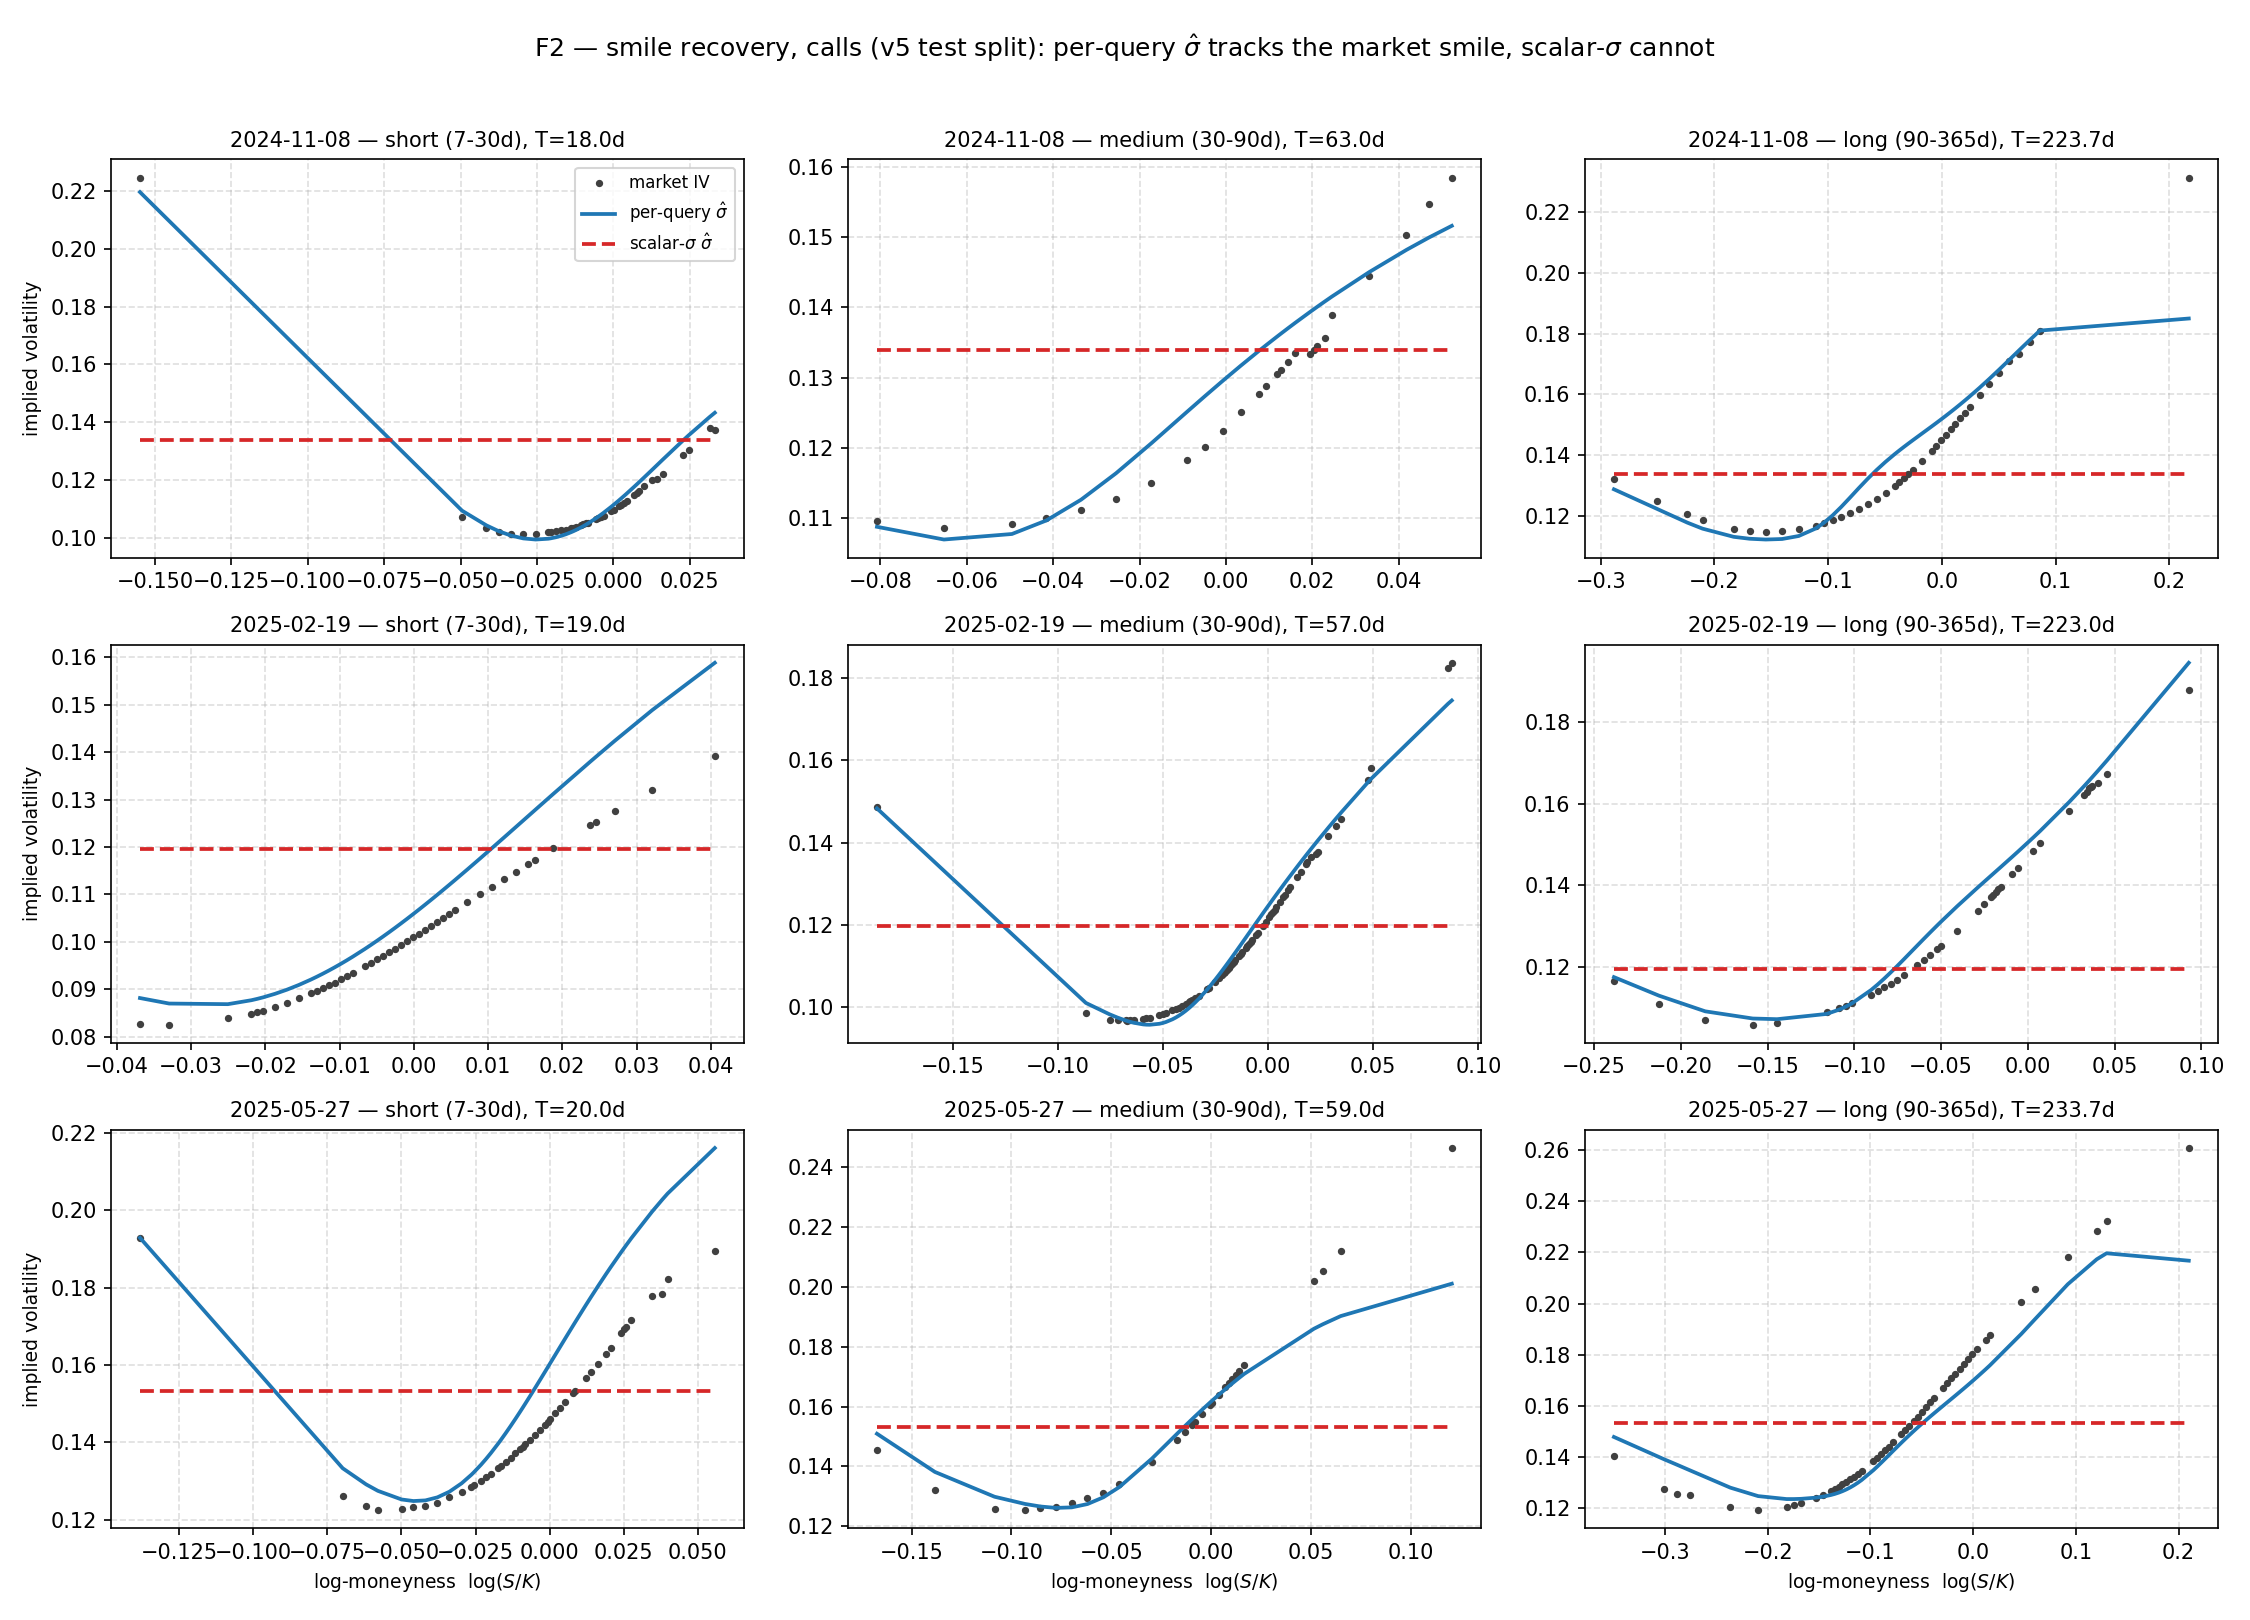
\includegraphics[width=\linewidth]{figures/fig_F2_smile_recovery_call_v5.png}
\caption{Calls}
\end{subfigure}
\begin{subfigure}[b]{\linewidth}
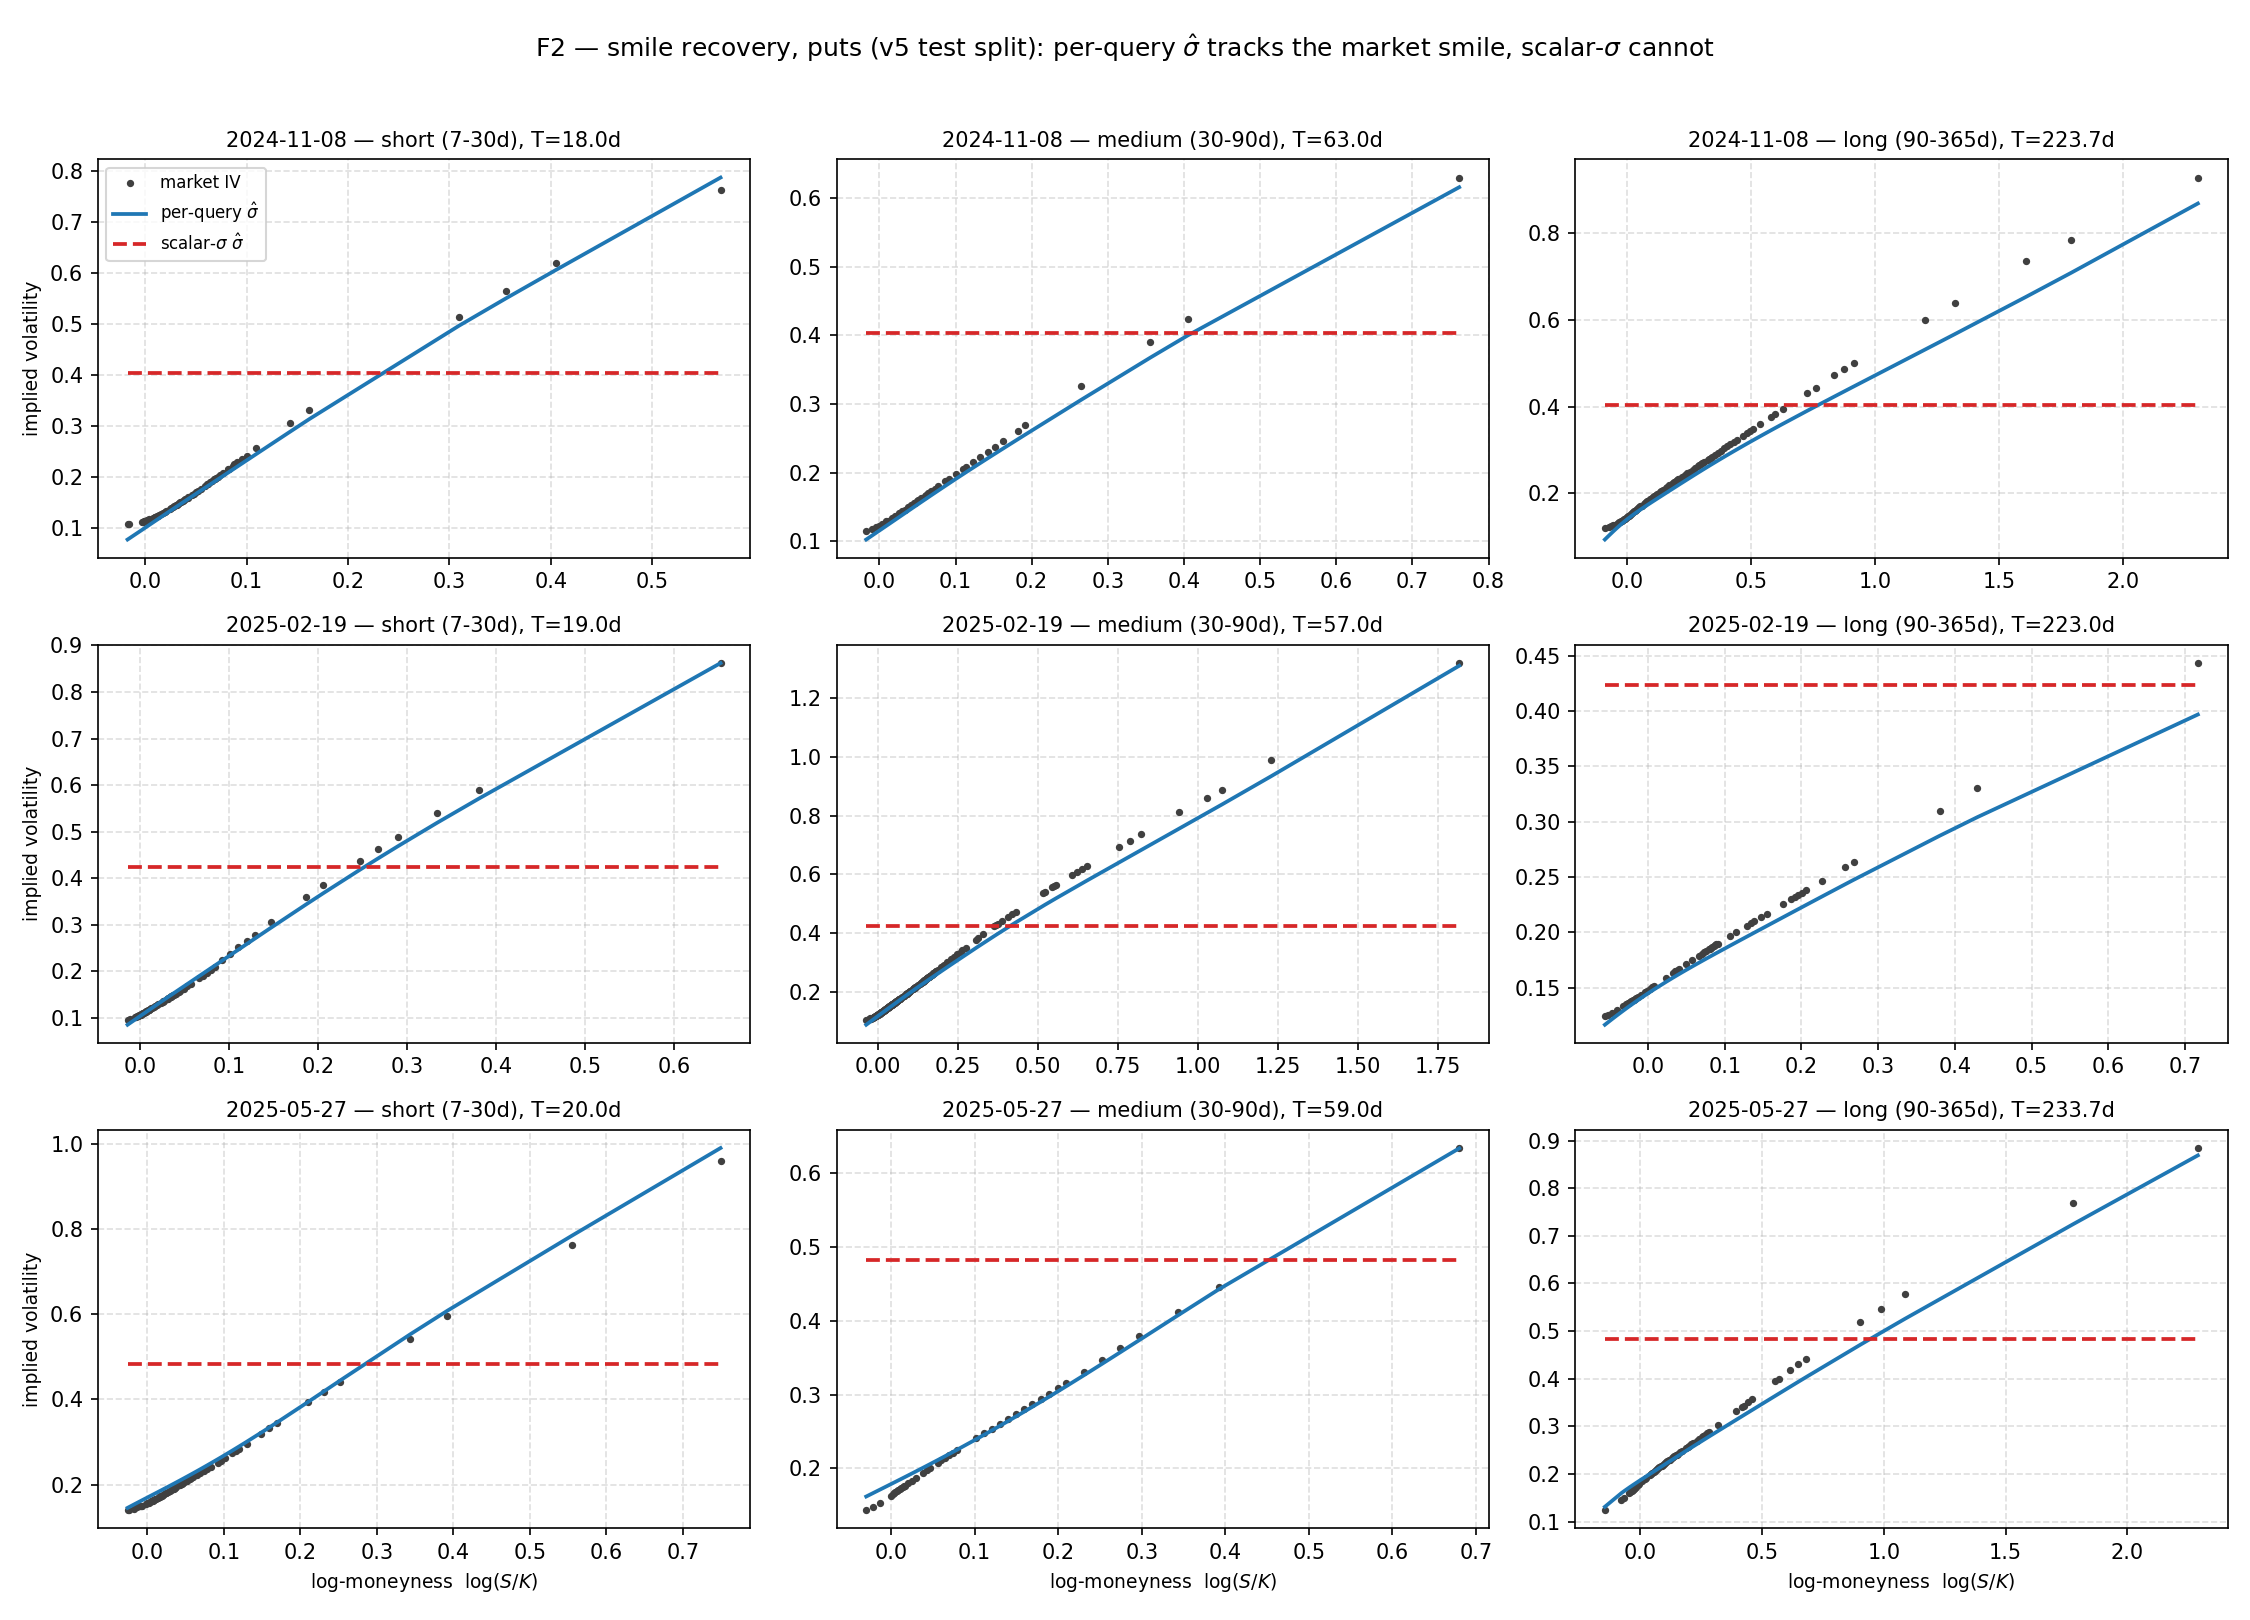
\includegraphics[width=\linewidth]{figures/fig_F2_smile_recovery_put_v5.png}
\caption{Puts}
\end{subfigure}
\caption{\textbf{Smile recovery on three test dates $\times$ three maturity buckets} (short 7--30d,
medium 30--90d, long 90--365d): market implied volatility, the per-query
$\hat\sigma(\text{latent}, \log m, T)$, and the scalar-$\hat\sigma$ control. The per-query curve tracks
the observed smile/skew in every panel; the scalar curve is flat by construction.}
\label{fig:f2}
\end{figure}

\subsection{Error stratification by moneyness and maturity}
\label{sec:results-error}
Figure~\ref{fig:f3} reports RMSE$(\log V/K)$ over a maturity $\times$ log-moneyness grid on the full
test split for the IV-surface, architecture-A models. Both option types show the same qualitative
pattern: error is highest in the deep out-of-the-money wings at short maturity and lowest near the
money at medium-to-long maturity. This residual near-expiry effect reflects a genuine, continuous
ill-conditioning of the inverse map $\log(\text{price}) \to \sigma$ as $T \to 0$, since the sensitivity
$\partial \log(\text{price})/\partial \hat\sigma$ shrinks near expiry and away from the money, not a
degenerate or unfittable region of the input: this dataset contains no contracts with $T \leq 1$ day by
construction, so the shortest surviving maturity band is simply where this continuous effect is most
visible, and on the price scale (rather than the log scale) the same cells are small in absolute terms.
The maturity-stratified rows of Figure~\ref{fig:f3} are how we report this near-expiry pattern; we do
not present a separate maturity-resolved tail plot.

\begin{figure}[t]
\centering
\begin{subfigure}[b]{0.48\linewidth}
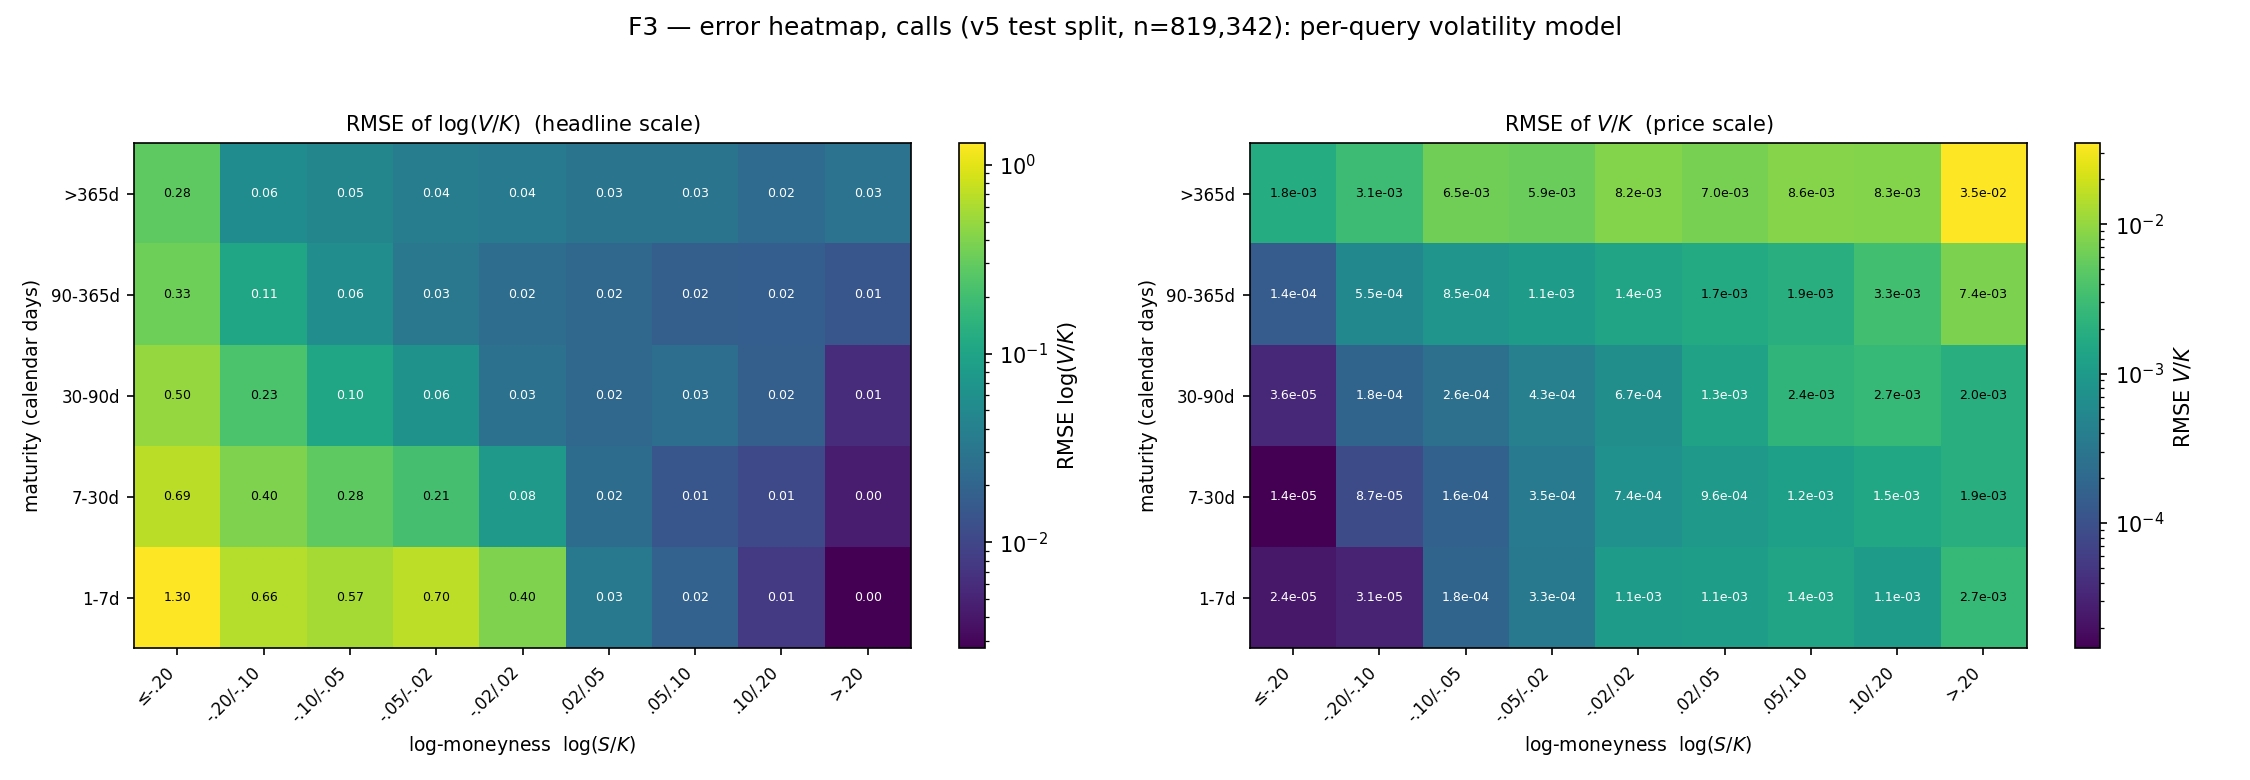
\includegraphics[width=\linewidth]{figures/fig_F3_error_heatmap_call_v5.png}
\caption{Calls}
\end{subfigure}
\hfill
\begin{subfigure}[b]{0.48\linewidth}
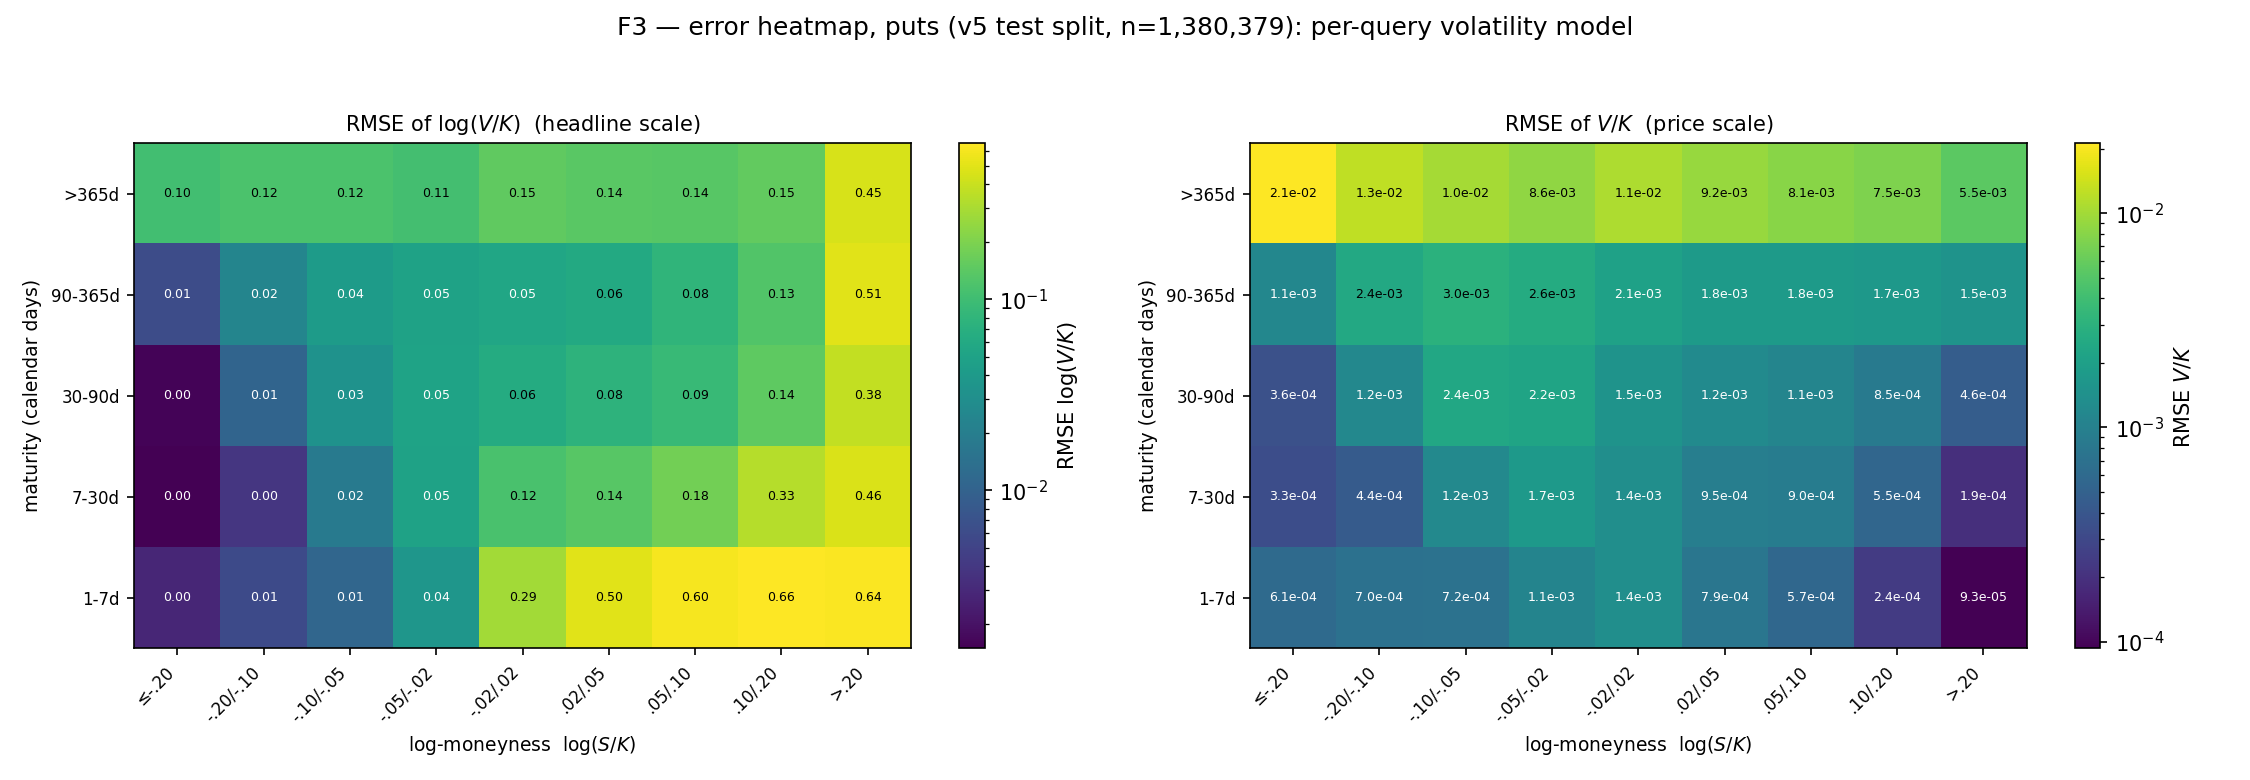
\includegraphics[width=\linewidth]{figures/fig_F3_error_heatmap_put_v5.png}
\caption{Puts}
\end{subfigure}
\caption{\textbf{RMSE($\log V/K$) over a $5 \times 9$ maturity $\times$ log-moneyness grid}, full test
split, IV-surface architecture-A models. Error is highest in the deep out-of-the-money wings at short
maturity and lowest near-the-money at longer maturity; the two grids mirror each other because a
call's out-of-the-money side is the opposite sign of log-moneyness from a put's.}
\label{fig:f3}
\end{figure}

\subsection{Comparison against baselines}
\label{sec:results-baselines}
Table~\ref{tab:baselines-call} and Table~\ref{tab:baselines-put} compare the best model against the
three baselines of Section~\ref{sec:baselines-method}.

\begin{table}[t]
\centering
\small
\caption{Calls: baselines are close to saturated on $R^2(\text{price})$; all five numbers lie within a
0.0014 range, so this metric alone does not discriminate pricers on this dataset. The log-space column
separates them sharply. Both constant-$\hat\sigma$ rows are train-subsample-fitted
(Section~\ref{sec:baselines-method}), one by
minimizing MSE on $\log(V/K)$ and one by minimizing MSE on $V/K$.}
\label{tab:baselines-call}
\begin{tabular}{lrr}
\toprule
Baseline / model & $R^2(\text{price})$ & $R^2(\log)$ \\
\midrule
Zero-volatility limit (discounted forward intrinsic) & 0.998586 & $-16.806016$ \\
Constant $\hat\sigma$, log-MSE fit ($\sigma{=}0.1933$) & 0.999706 & 0.620788 \\
Constant $\hat\sigma$, price-MSE fit ($\sigma{=}0.1761$) & 0.999800 & 0.640351 \\
IV-surface spline interpolation & 0.999982 & 0.764181 \\
Best neural model (IV surface, A) & 0.999977 & \textbf{0.991044} \\
\bottomrule
\end{tabular}
\end{table}

\begin{table}[t]
\centering
\small
\caption{Puts: price-space and log-space metrics disagree on which pricer wins. Both
constant-$\hat\sigma$ rows are train-subsample-fitted (Section~\ref{sec:baselines-method}), one by
minimizing MSE on $\log(V/K)$ and
one by minimizing MSE on $V/K$; the two objectives select different constants and rank in opposite
directions on the two metrics.}
\label{tab:baselines-put}
\begin{tabular}{lrr}
\toprule
Baseline / model & $R^2(\text{price})$ & $R^2(\log)$ \\
\midrule
Zero-volatility limit (discounted forward intrinsic) & 0.535219 & $-34.203142$ \\
Constant $\hat\sigma$, log-MSE fit ($\sigma{=}0.4758$) & $-2.358206$ & $-0.388064$ \\
Constant $\hat\sigma$, price-MSE fit ($\sigma{=}0.2063$) & 0.925761 & $-3.358130$ \\
IV-surface spline interpolation & 0.996594 & $-2.518559$ \\
Best neural model (IV surface, B) & 0.993780 & \textbf{0.981298} \\
\bottomrule
\end{tabular}
\end{table}

On calls, all five numbers in Table~\ref{tab:baselines-call} sit within a 0.0014 range: the
zero-volatility limit, with no fitted parameters, already reaches $R^2(\text{price}) = 0.9986$, so
call price-$R^2$ is a weak discriminator on its own and the log-space metric is the more informative
one for calls. That column separates the same pricers cleanly: $-16.81$ for the zero-volatility limit,
0.621 and 0.640 for the log-fitted and price-fitted constant $\hat\sigma$, 0.764 for spline
interpolation of the observed surface, and 0.991 for the model. Unlike puts, calls show no material
metric disagreement: the model leads every baseline on log-space and sits within $6\times10^{-6}$ of
the best baseline on price-space (a gap of $5.5\times10^{-6}$). On puts, the two metrics disagree on
which pricer wins: IV-surface spline interpolation edges out the model on price-space (0.996594 vs.\
0.993780), while the model leads on log-space by 3.50 in $R^2$ (0.981298 vs.\ $-2.518559$).
Whichever pricer a reader considers ``better'' for puts depends on which metric they weight; we
report both rather than only the more flattering one.

The spline's negative put log-$R^2$ is a grid-boundary artefact rather than a general failure of
surface interpolation. A row-level decomposition of the same baseline
(\texttt{analysis/spline\_boundary\_decomposition.py}, which reproduces the aggregate $R^2$ of
Table~\ref{tab:baselines-put} to $10^{-6}$) finds that 578{,}610 of the 1{,}380{,}379 put test rows
(41.92\%) converge to $|\delta|$ below the surface's 10-delta boundary and are therefore all priced off
that one clamped column. Those rows carry 99.94\% of the spline's log-space sum of squared errors and
all 272{,}433 squared-log errors above 10, while the rows clamped on neither axis reach
$R^2(\log) = 0.9939$ (0.9843 on the looser reading that excludes only the delta clamp and keeps
tenor-clamped rows). The mechanism is a scale mismatch between the two metrics: clamping a deep
out-of-the-money put to the 10-delta implied volatility is a large multiplicative error, but it acts on
a small normalized price, the mean true $V/K$ on those rows being 0.00203 against 0.0202 in-grid and
0.0886 deep in the money. They still carry 72.94\% of the price-space sum of squared errors, a
substantial share and not a negligible one, but $R^2(\text{price})$ is scored against a variance
denominator that the in-the-money rows set, and that denominator is large enough to leave it at
0.996594. Calls show the same structure more weakly, with 185{,}863 rows (22.68\%) below 10 delta
carrying 99.40\% of call log-space SSE. This is also where the learned model's log-space advantage over
interpolation is concentrated, since the standardized surface has no support beyond 10 delta; the
model's own error heatmap (Figure~\ref{fig:f3}) places its worst cells in the same wings, so the
advantage there is relative rather than absolute.

The put constant-$\hat\sigma$ baseline depends strongly on the objective it was fitted under, so what
ranks it is the choice of fitting space and not the constancy of $\hat\sigma$ alone. Fitted by
minimizing MSE on $\log(V/K)$ it selects $\sigma = 0.4758$ and scores below the zero-volatility limit
on put price-space ($-2.358206$ vs.\ 0.535219); fitted by minimizing MSE on $V/K$ it selects
$\sigma = 0.2063$ and reaches $R^2(\text{price}) = 0.925761$, but falls to $R^2(\log) = -3.358130$. The
log-space objective is dominated by deep out-of-the-money puts, whose implied volatilities are the
highest in the cross-section, so the constant it selects is far too high for near-the-money puts and
overprices them badly on the price scale, where those contracts carry almost all of the variance. The
price-fitted constant reverses the picture, pricing the near-the-money contracts acceptably at the cost
of the wings that dominate the log metric. The claim is therefore narrow: it is the log-fitted constant
that scores below the zero-volatility limit on put price-space, not any single global volatility.

Figure~\ref{fig:f5} shows predicted-vs-market price scatter on a 50{,}000-row uniform sample of the
test split. Calls reach $R^2(\text{price}) = 0.999954$, Pearson correlation (log-log) $r = 0.995619$,
median relative error 3.61\%, and 76.62\% of rows within $\pm 10\%$. Puts reach
$R^2(\text{price}) = 0.993179$, $r = 0.991166$, median relative error 8.74\%, and 54.46\% of rows within
$\pm 10\%$.

\begin{figure}[t]
\centering
\begin{subfigure}[b]{0.48\linewidth}
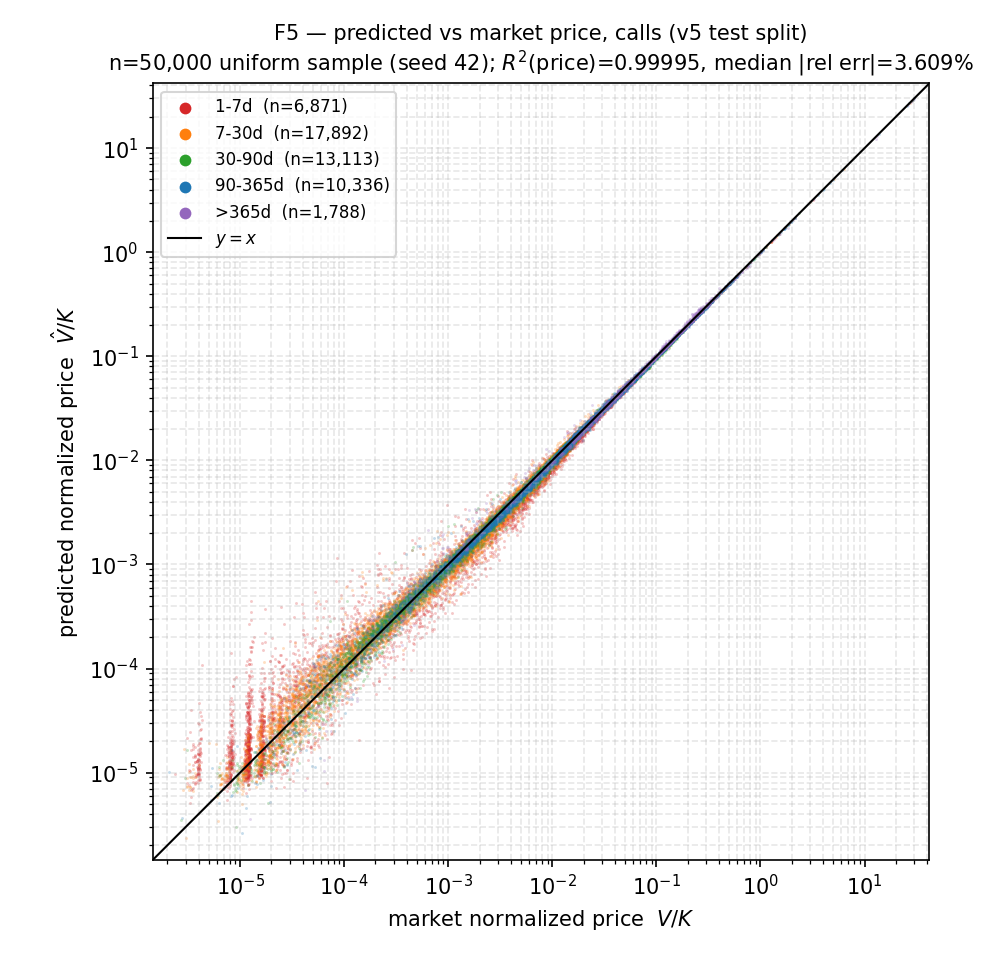
\includegraphics[width=\linewidth]{figures/fig_F5_pred_vs_market_call_v5.png}
\caption{Calls}
\end{subfigure}
\hfill
\begin{subfigure}[b]{0.48\linewidth}
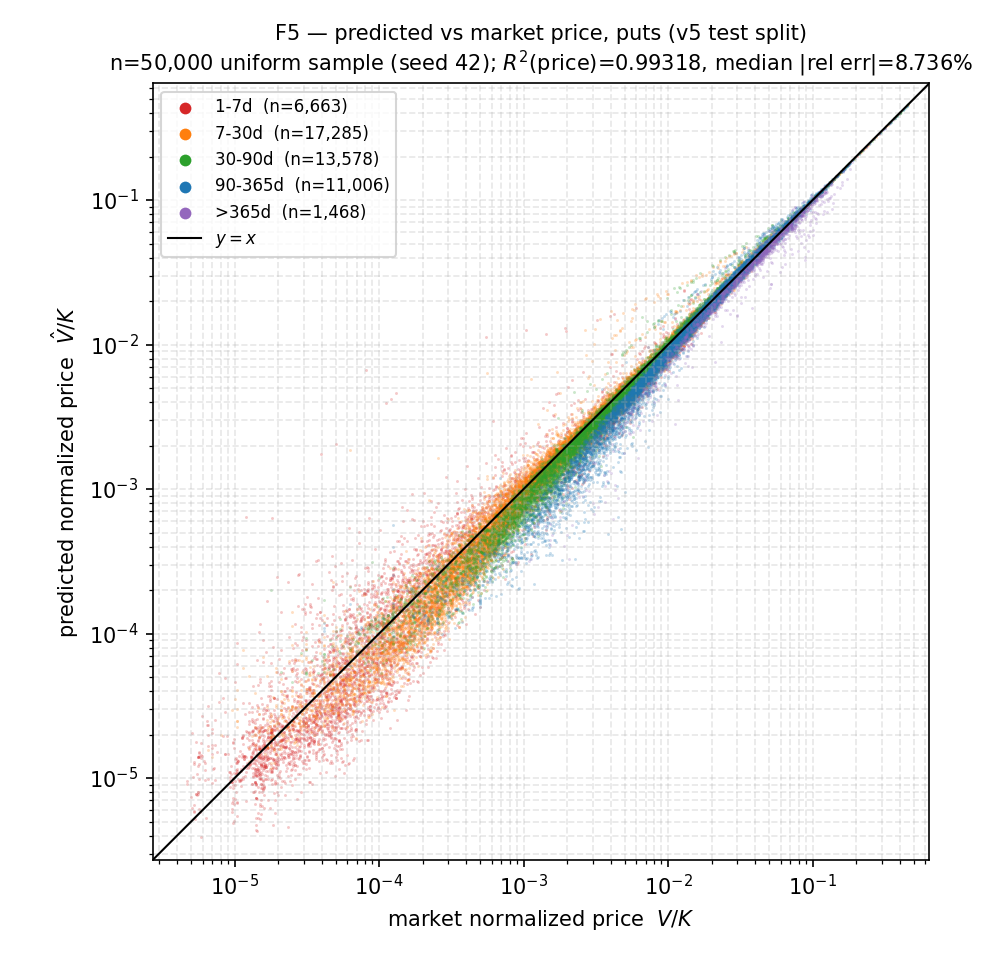
\includegraphics[width=\linewidth]{figures/fig_F5_pred_vs_market_put_v5.png}
\caption{Puts}
\end{subfigure}
\caption{\textbf{Predicted vs.\ market normalized price ($V/K$)}, log-log axes, colored by maturity
bucket, 50{,}000-row uniform sample of the test split, IV-surface architecture-A models.}
\label{fig:f5}
\end{figure}

\subsection{Black--Scholes decoder derivative consistency}
\label{sec:results-greeks}
Table~\ref{tab:greeks} reports the agreement between autograd-computed and closed-form delta and vega
at the predicted $\hat\sigma$, over 2{,}000 sampled test contracts per option type.

\begin{table}[t]
\centering
\small
\caption{Decoder derivative-consistency check: autograd vs.\ closed-form BS partial greeks at the
predicted $\hat\sigma$, held fixed. $n{=}2{,}000$ sampled test contracts per option type.}
\label{tab:greeks}
\begin{tabular}{lrrrr}
\toprule
Option & Delta max abs.\ diff. & Delta median abs.\ diff. & Vega max abs.\ diff. & Vega median abs.\ diff. \\
\midrule
Call & $1.84\times10^{-14}$ & $1.40\times10^{-16}$ & $1.38\times10^{-15}$ & $5.55\times10^{-17}$ \\
Put  & $1.43\times10^{-14}$ & $8.37\times10^{-17}$ & $2.12\times10^{-15}$ & $5.55\times10^{-17}$ \\
\bottomrule
\end{tabular}
\end{table}

Agreement is at float64 machine precision, as expected for two mathematically identical expressions
evaluated by two different computational paths. The largest absolute discrepancy over the sampled
contracts is $1.84\times10^{-14}$ for call delta and $1.43\times10^{-14}$ for put delta, and
$1.38\times10^{-15}$ for call vega and $2.12\times10^{-15}$ for put vega, with medians at or below
$1.40\times10^{-16}$; we quote the two greeks separately rather than as a single range, since their
maxima differ by an order of magnitude. This confirms the decoder is implemented and
differentiated correctly at the predicted $\hat\sigma$; it is not an independent check of the learned
$\hat\sigma$ itself, and it does not measure the total (sticky-strike) sensitivity of the learned
system, which would include a $\partial \hat\sigma/\partial S \cdot \text{vega}$ term this
frozen-$\hat\sigma$ check does not exercise.

\section{Limitations}
\label{sec:limitations}

The results above are bounded by several scope limits that we state explicitly rather than leave
implicit.

\paragraph{Pointwise, not surface-wide, Black--Scholes consistency.} At a fixed predicted $\hat\sigma$,
the decoder guarantees the single-contract static no-arbitrage bounds at each queried contract, but not
calendar-spread or butterfly consistency across the predicted surface, and not that the total learned
map, in which $\hat\sigma$ varies with the query, satisfies the BS PDE. A violation-rate diagnostic on
the predicted $(K,T)$ surface would be needed to make a surface-wide claim, and we do not run one here.

\paragraph{Call price-$R^2$ is a weak metric on this dataset.} The zero-volatility limit (discounted
forward intrinsic), which fits no parameter, already reaches $R^2(\text{price}) = 0.9986$ for calls
(Table~\ref{tab:baselines-call}), so most of the call price-$R^2$ figures in this paper should not be
read as strong evidence on their own; the put comparison and the log-space metric carry the
informative signal.

\paragraph{The put interpolation comparison is shaped by grid clamping.} The spline baseline's negative
put log-$R^2$ comes almost entirely from rows clamped to the standardized surface's 10-delta boundary
(Section~\ref{sec:results-baselines}), so it measures a limit of that grid's support rather than an
absence of information in the observed surface. Reading the model's log-space lead over interpolation
as a statement about surface-based pricing in general would require a comparator that extrapolates
beyond the grid, such as an SVI or SSVI fit~\citep{Gatheral2004SVI,GatherJacquier2014SSVI}, which we do
not evaluate here.

\paragraph{Architecture ranking (A vs.\ B) is underdetermined.} Three-seed replication exists only for
the four IV-surface cells, and even there the put result, B somewhat ahead of A, rests on three seeds,
not enough for a superiority claim; we report descriptive across-seed dispersion and run no
inferential test anywhere in this paper. The SPX-history and VIX-history branches are single-seed
throughout, with genuinely unmeasured dispersion, so we make no architecture claim for those eight
cells. The scalar-$\hat\sigma$ ablation is likewise single-seed (Section~\ref{sec:ablation-method}), so
its magnitudes describe one run.

\paragraph{The surface branch is conditioned on same-day information.} Its input is OptionMetrics' own
standardized surface for the trade date being priced, built from that day's quotes
(Section~\ref{sec:data-surface}). The date-based split removes cross-date leakage but not this
within-date dependence, so the surface-branch results establish same-day cross-sectional reconstruction
conditional on an observed surface, not forecasting or independent price discovery; any deployment
reading of those numbers would require the surface to be available at pricing time. The historical
branches are not strictly-prior-information inputs either: their 21-trading-day windows end on the
target trade date and are normalized by that day's close, and VIX is itself computed from
contemporaneous SPX option quotations. Their same-day option-market content is far smaller and less
direct than the surface branch's, but a design that required strictly pre-trade-date information would
have to lag these windows by a day, which we did not do.

\paragraph{The branch comparison compares configurations, not inputs, and the VIX representation is
level-free.} The first, grid-dependent layer of the two-layer flattening projection holds 766{,}080
(surface), 430{,}208 (SPX history), and
344{,}192 (VIX history) parameters, a spread of roughly $2.2\times$; grid size, spectral modes, input
timing, and normalization also differ across the three branches. Input content is therefore confounded
with all of these in Section~\ref{sec:results-branch}, and the result should be read as a ranking of
three whole input--encoder configurations rather than an isolation of input content. Separately, the
VIX-history tensor is divided by the window's final VIX close, which discards the absolute VIX level
and retains only the path shape, so the VIX result speaks only to that close-normalized representation
and not to VIX history as an information source. A capacity-matched rerun with a level-preserving VIX
encoding would be needed to attribute the branch gap to input content alone.

\paragraph{Near-expiry ill-conditioning is real and not removed by the maturity filter.} The maturity
filter removes the degenerate exact-$T{=}0$ case but not the continuous ill-conditioning of
$\partial \log(\text{price})/\partial \hat\sigma$ as $T \to 0$; the shortest surviving maturity band
still shows elevated log-space error (Section~\ref{sec:results-error}), though it is small in absolute
price terms.

\paragraph{Single underlying, European exercise only.} All results are on SPX index options. European
exercise removes the early-exercise complication, and BS is used as the analytical decoder, with the
dividend yield handled through the decoder's $q$ term. We make no claim about American-style contracts
or other underlyings, and the remaining BS idealizations, constant volatility over the contract's life
and frictionless continuous trading, are not satisfied by the market; this is precisely why $\hat\sigma$
must be predicted per contract in the first place.

\paragraph{Mid-price only.} We price the bid-ask midpoint; transaction costs and the bid-ask spread
itself are out of scope.

\paragraph{No direct-price-regressor control.} We do not compare against a direct-price regressor of
comparable size that skips the BS decoder entirely, so this paper makes no claim about how the
BS-decoder design compares to that alternative.

\section{Conclusion}
\label{sec:conclusion}
Predicting a per-contract implied volatility and pricing it through a differentiable Black--Scholes
decoder removes the need for a learned pricing surrogate. Conditional on the predicted $\hat\sigma$
being held fixed, this yields two structural properties by construction: analytic partial greeks at
that $\hat\sigma$, with autograd through the decoder and closed-form BS agreeing to a maximum absolute
discrepancy of approximately $2\times10^{-14}$ for delta and $2\times10^{-15}$ for vega
(Section~\ref{sec:results-greeks}), and pointwise Black--Scholes-consistent
prices at every queried contract (Section~\ref{sec:method-decoder}). Neither extends to the total
learned map, whose $\hat\sigma$ varies with the query, nor to arbitrage-freedom across the full
predicted surface.

The per-query-vs-scalar ablation (Section~\ref{sec:results-ablation}) shows that per-query conditioning
matters: removing it collapses put $R^2(\log)$ from 0.978 to about $-0.32$ and put $R^2(\text{price})$ to
$-3.09$, worse than predicting the mean. Comparing three candidate market-state input--encoder
configurations, the one reading the contemporaneous implied-volatility surface consistently prices
better than either historical configuration, on both option types and both head architectures
(Section~\ref{sec:results-branch}). The surface-branch models were stable across three seeds, and the
observed seed-42 gap between the surface configuration and the historical ones is much larger than the
surface branch's own seed-to-seed dispersion; full robustness of the branch-versus-branch comparison
cannot be established without also replicating the SPX-history and VIX-history runs, which remain
single-seed. That comparison is not, however, like-for-like: the surface branch reads OptionMetrics'
own same-day standardized surface, so it demonstrates out-of-time (date-split), same-day cross-sectional
reconstruction conditional on an observed surface rather than forecasting, and the three encoders
differ in grid size, normalization, and parameter count while the VIX input is normalized in a way that
removes the absolute VIX level (Section~\ref{sec:limitations}). The separate question of which
per-query head architecture is better remains unresolved: the observed differences are small relative
to the seed-to-seed variation we measure, and three seeds are insufficient to rank them.

Taken together, on this dataset the approach reaches $R^2(\text{price}) \approx 0.9999$--$0.99998$ and
$R^2(\log) \approx 0.990$--$0.991$ on the IV-surface input for calls, though calls' price-$R^2$ is close
to the zero-volatility limit and should not be read in isolation. The more informative put comparison
shows the model 0.003--0.004 below IV-surface interpolation on price-space (0.993--0.994 vs.\ 0.997)
but ahead of it by roughly 3.5 in $R^2(\log)$ (0.978--0.981 vs.\ $-2.52$), a gap that the
grid-boundary decomposition of Section~\ref{sec:results-baselines} attributes to clamping at the
surface's 10-delta edge.

% Acknowledgments section intentionally omitted: no funding to acknowledge for this draft.
% Add a \section*{Acknowledgments} block here before submission if that changes.

\bibliographystyle{plainnat}
\bibliography{references}

\appendix

\section{Hyperparameters}
\label{app:hyper}
Identical across all twelve core runs: seed 42 (plus seeds 43, 44 for the four IV-surface replication
runs); Adam phase, 100 epochs, learning rate $10^{-3}$ with reduce-on-plateau scheduling; fine-tuning
phase, 50 epochs, learning rate $10^{-5}$, minimum 10 fine-tuning epochs; batch size 256,
gradient-norm clipping at 1.0; early-stopping patience 5 in each phase. The FNO encoder uses 4 spectral
convolution blocks with $1{\times}1$-convolution skip connections and SiLU activations, width 32,
flattened and projected to a 128-dimensional latent/basis vector; head/trunk hidden width is 128. The
number of retained spectral modes follows the grid: $4 \times 8$ (modes1 $\times$ modes2) for the
surface encoder on its $11 \times 17$ grid, and $6 \times 2$ for both the SPX-history ($21 \times 5$)
and VIX-history ($21 \times 4$) encoders.
Architecture B (DeepONet) additionally uses a small positive $\hat\sigma$ floor and a learned scalar
bias initialized so that $\hat\sigma \approx 0.20$ at initialization.

\section{Numerical stability}
\label{app:numstab}
The default training and evaluation path computes $\log(\mathrm{clamp}(V/K, 10^{-8}))$ for numerical
stability. A numerically exact alternative, using a stable log-normal-CDF formulation, is available for
evaluation only: its gradient is exact but explodes near the money, which causes training to diverge if
used during optimization, so it is used only as a read-only diagnostic, never during training.

A controlled re-evaluation of the same scalar-$\hat\sigma$ checkpoints on CPU (batch 512 and 4096) and
GPU (batch 512, the training-time path) reproduces $R^2(\text{price})$ to within $4\times10^{-7}$ but
$R^2(\log)$ only to about $3\times10^{-3}$ across device paths, and decoding the same float32
$\hat\sigma$ in float64 moves $R^2(\log)$ further, to 0.798 for calls and $-0.328$ for puts, because
cancellation in the float32 Black--Scholes decoder, before the $10^{-8}$ price clamp and logarithm,
moves near-zero predictions on and off the clamp floor across device paths and precisions; the
per-query models, which never reach the floor, differ by at most $1.5\times10^{-6}$ in $R^2(\log)$
across the evaluated paths and precisions
(\texttt{results/ablation\_evaluator\_consistency\_v5.json}). The scalar-$\hat\sigma$ log-space metrics
are therefore stable only to about $10^{-2}$ in $R^2(\log)$ for puts and $2\times10^{-3}$ for calls,
which is why the prose reports them to two decimals; Table~\ref{tab:ablation} keeps the canonical
float32 CPU evaluator's digits. No implementation error was found.

\section{Reproducibility and environment}
\label{app:repro}
Table~\ref{tab:env} records the environment captured on 2026-09-07 by
\texttt{analysis/snapshot\_environment.py}
(\texttt{results/environment\_snapshot\_2026-09-07.txt}) and used for the publication-audit
diagnostics described above. The August 2026 training environment was not snapshotted, and this table
should not be interpreted as reconstructing either the training environment or every earlier
evaluation run.

\begin{table}[H]
\centering
\small
\caption{Environment captured 2026-09-07 and used for the publication-audit diagnostics. It is
neither the training environment nor necessarily that of every earlier evaluation run.}
\label{tab:env}
\begin{tabular}{ll}
\toprule
Component & Version \\
\midrule
Python & 3.11.15 \\
PyTorch & 2.10.0 (built against CUDA 13.0) \\
NumPy & 2.3.5 \\
h5py & 3.16.0 \\
matplotlib & 3.10.8 \\
polars & 1.38.1 \\
GPU & NVIDIA GeForce RTX 3060 \\
GPU driver & 595.95 \\
\bottomrule
\end{tabular}
\end{table}

Each run's exact configuration is saved alongside its checkpoints at training time; that record covers
the seed, the hyperparameters, and the dataset version and checksum, but not package versions.

\end{document}
